\documentclass[12pt]{article}
\usepackage[a4paper, margin=1in]{geometry} 
\usepackage{graphicx} 
\usepackage{hyperref}
\usepackage{float}
\usepackage{multicol}
\usepackage{multirow}
\usepackage{amsmath}
\usepackage[ruled]{algorithm2e}
\usepackage{amssymb}
\usepackage[font=small, labelfont=bf]{caption}
\usepackage[table,xcdraw]{xcolor}

\title{Lecture Notes for \\ INF281 Basics of Bioinformatics Sequence Analysis}
\author{Takaya Saito}
\date{}

\begin{document}

\clearpage\maketitle
\vspace{450px}

\includegraphics[scale=1]{fig00/88x31.png} \\
This work is licensed under a Creative Commons Attribution 4.0 International License.
\thispagestyle{empty}
\pagebreak

\pagenumbering{roman}
\setcounter{page}{1}
\tableofcontents
\pagebreak

\pagenumbering{arabic}
\setcounter{page}{1}

\makeatletter 
\renewcommand{\thefigure}{\arabic{section}.\arabic{figure}}
\renewcommand{\thetable}{\arabic{section}.\arabic{table}}
\makeatother

%
% PART I
%
\part{}

%
% Introduction
%
\setcounter{figure}{0}
\setcounter{table}{0}
\section{Introduction}
%\documentclass[12pt]{article}
%\usepackage[a4paper, margin=1in]{geometry} 
%\usepackage{graphicx} 
%\usepackage{hyperref}
%\usepackage{float}
%\usepackage[font=small, labelfont=bf]{caption}
%
%\begin{document}

%
% Introduction to Molecular Biology
%
\subsection{Introduction to Molecular Biology}
Molecular biology is the study of biology focusing on organisms and cells at the molecular level.

%
% Five essential facts about cells
%
\subsubsection*{Five essential facts about cells}

\textbf{1. Two primary types of cells –- eukaryotes and prokaryotes}
\begin{itemize}
\item Eukaryote: animals \& plants
\item Prokaryote: bacteria \& archaea
\end{itemize}
\begin{figure}[H]
  \centering
      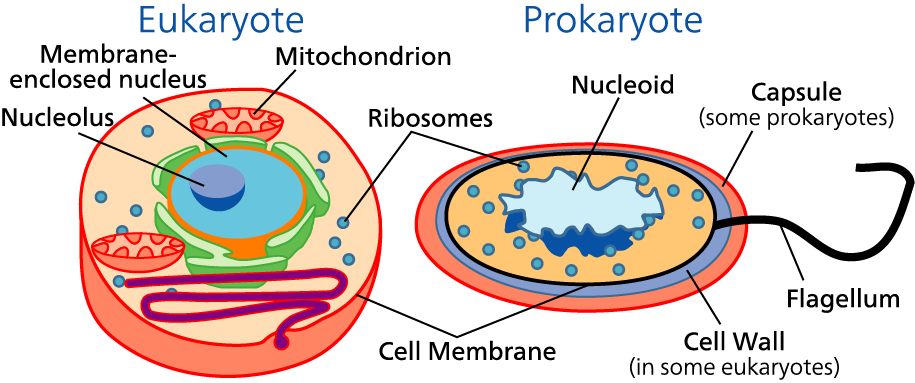
\includegraphics[width=0.75\textwidth]{fig01/prokaryote_and_eukaryote_cells.png}
  \caption{Eukaryotic and prokaryotic cells (source: \href{https://commons.wikimedia.org/wiki/File:Celltypes.svg}{Science Primer, Wikimedia Commons})}
\end{figure}

\noindent \textbf{2. Cell size –- around 1 to 100 micrometers}
\begin{itemize}
\item Cell Size and Scale: \url{http://learn.genetics.utah.edu/content/cells/scale}
\end{itemize}
\medskip  

\noindent \textbf{3. The number of cells}
\begin{itemize}
\item Prokaryotes: 1 cell
\item Human:  Estimate of 15 trillion cells
\end{itemize}
\medskip 

\noindent \textbf{4. An animal cell and cell organelles}
\begin{figure}[H]
  \centering
      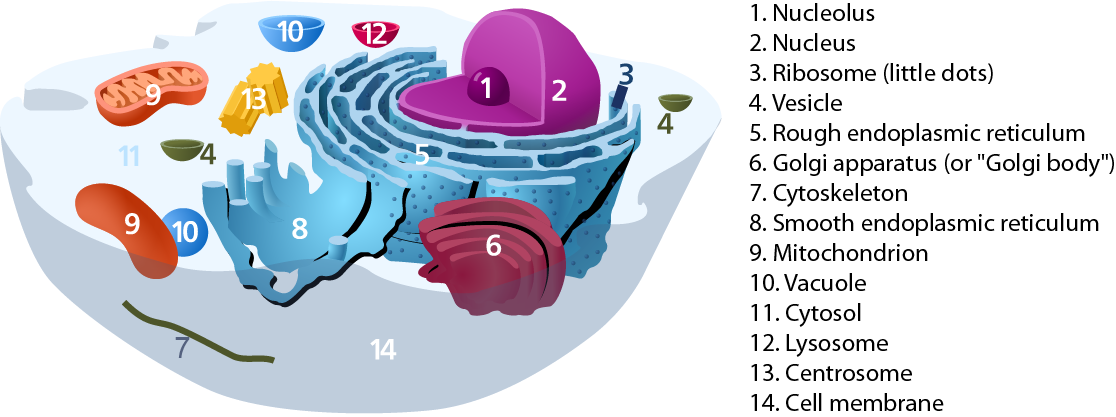
\includegraphics[width=0.75\textwidth]{fig01/animal_cells_and_organelles.png}
  \caption{An animal cell and organelles (source: \href{https://en.wikipedia.org/wiki/Organelle\#/media/File:Animal_Cell.svg}{Kelvinsong, Wikimedia Commons})}
\end{figure}

\noindent \textbf{5. Cellular processes}
\begin{itemize}
\item Cell growth, cell development, cell signaling, …
\item Example: \url{http://www.nature.com/nrg/multimedia/rnai}
\end{itemize}

%
% Central dogma of molecular biology
%
\subsubsection*{Central dogma of molecular biology}

It describes the information flow within a cell.

\begin{figure}[H]
  \centering
      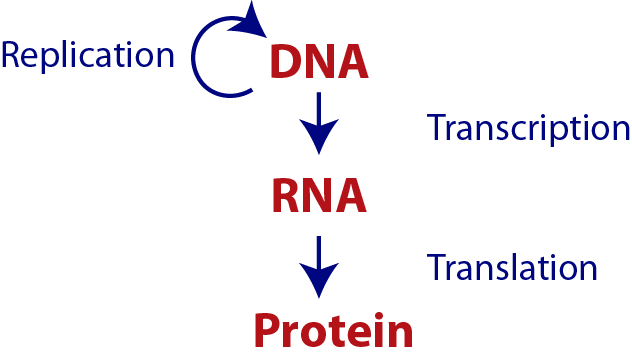
\includegraphics[width=0.75\textwidth]{fig01/central_dogma_of_molecular_biology.png}
  \caption{Central dogma of molecular biology}
\end{figure}

%
% DNA (deoxyribonucleic acid)
%
\subsubsection*{DNA (deoxyribonucleic acid)}

DNA stores genetic information. It has four different bases: cytosine (C), guanine (G), adenine (A), and thymine (T).

\begin{figure}[H]
  \centering
      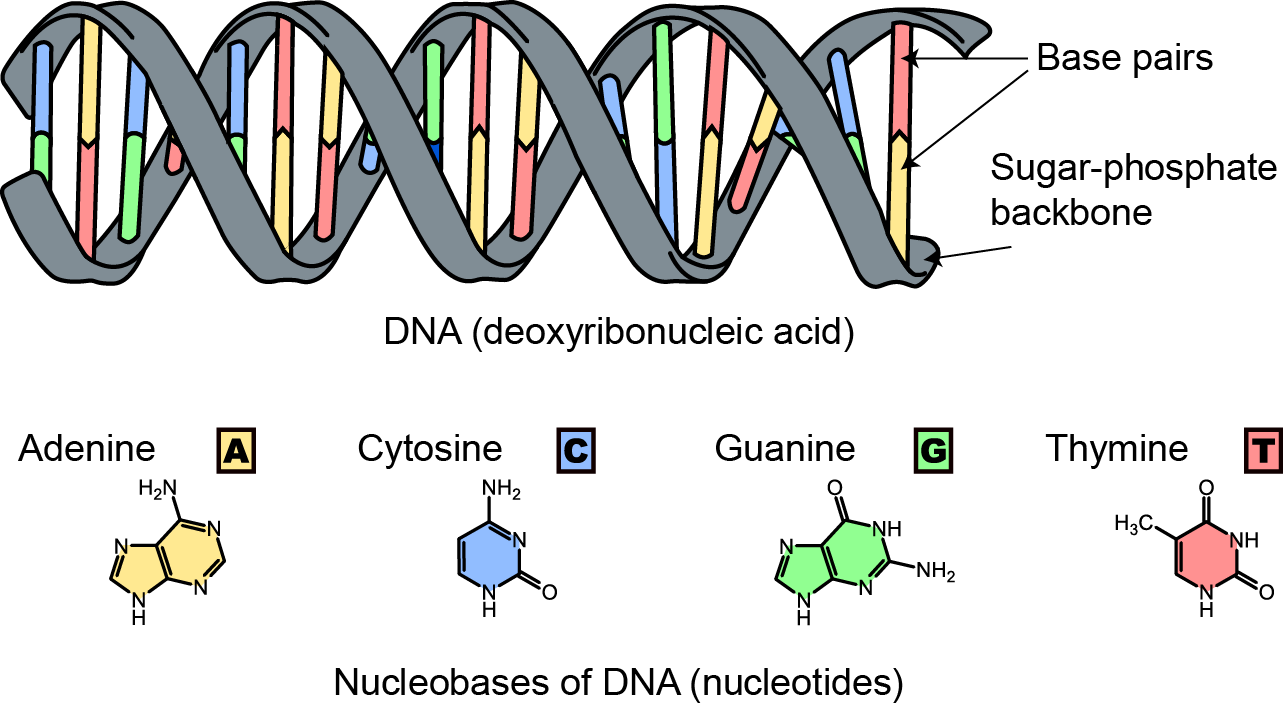
\includegraphics[width=0.5\textwidth]{fig01/dna_bases.png}
  \caption{DNA double helix and base pairs \newline (modified from the original version by \href{https://commons.wikimedia.org/w/index.php?curid=9810855}{Sponk, Wikimedia Commons})}
\end{figure} 

\noindent \textbf{Base pair matching (Watson-Crick base pair)}

\noindent Adenine (A) pairs with thymine (T), whereas cytosine (C) pairs with guanine (G).

\begin{verbatim}
DNA strand1: ACGT
             ||||
DNA strand2: TGCA
\end{verbatim}
	
%
% RNA (Ribonucleic acid)
%
\subsubsection*{RNA (Ribonucleic acid)}
RNA has various biological roles and several sub-classes. Messenger RNAs (mRNAs) convey genetic information.  It has four different bases: cytosine (C), guanine (G), adenine (A), and uracil (U).

\begin{figure}[H]
  \centering
      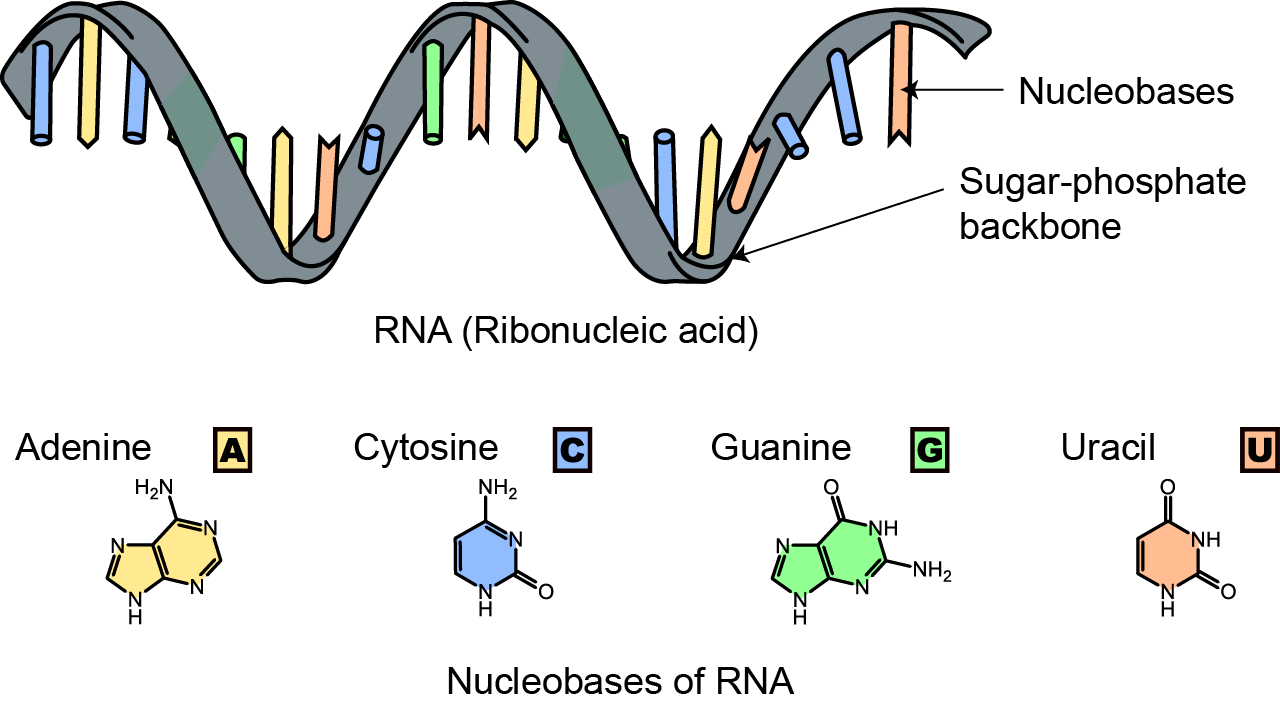
\includegraphics[width=0.5\textwidth]{fig01/rna_bases.png}
  \caption{Single strand RNA \newline (modified from the original version by \href{https://commons.wikimedia.org/w/index.php?curid=9810855}{Sponk, Wikimedia Commons})}
\end{figure}

\noindent \textbf{Transcription: mRNAs are transcribed from DNAs}

\begin{verbatim}
DNA: ACGT -------> RNA: ACGU
        Transcription
\end{verbatim}

%
% Protein
%
\subsubsection*{Protein}

Proteins are large molecules consisting of amino acids. There are 20 common amino acids.
 
\begin{figure}[H]
  \centering
      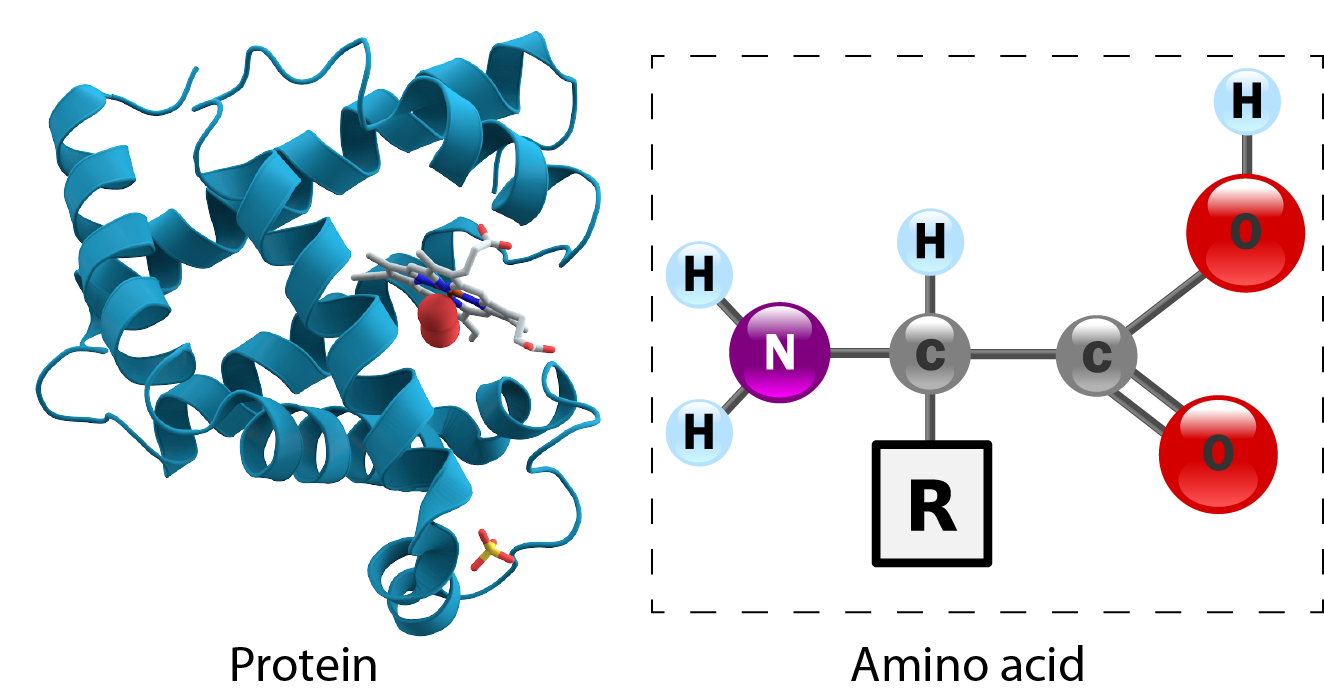
\includegraphics[width=0.6\textwidth]{fig01/protein_and_amino_acid.png}
  \caption{Protein 3D structure and amino acids \newline (sources: \href{https://en.wikipedia.org/wiki/Protein\#/media/File:Myoglobin.png}{AzaToth, Wikimedia Commons}, \href{https://en.wikipedia.org/wiki/Amino_acid\#/media/File:AminoAcidball.svg}{YassineMrabet, Wikimedia Commons})}
\end{figure}

\noindent \textbf{Translation: Amino-acids are translated from mRNAs}

\begin{verbatim}
mRNA: GUC -------> AA: Valine
        Translation
\end{verbatim}

\newpage 

\noindent \textbf{Universal genetic code}

\noindent A codon consists of three nucleic acids. Single-letter or three-letter names can be used for amino acids.

\begin{figure}[H]
  \centering
      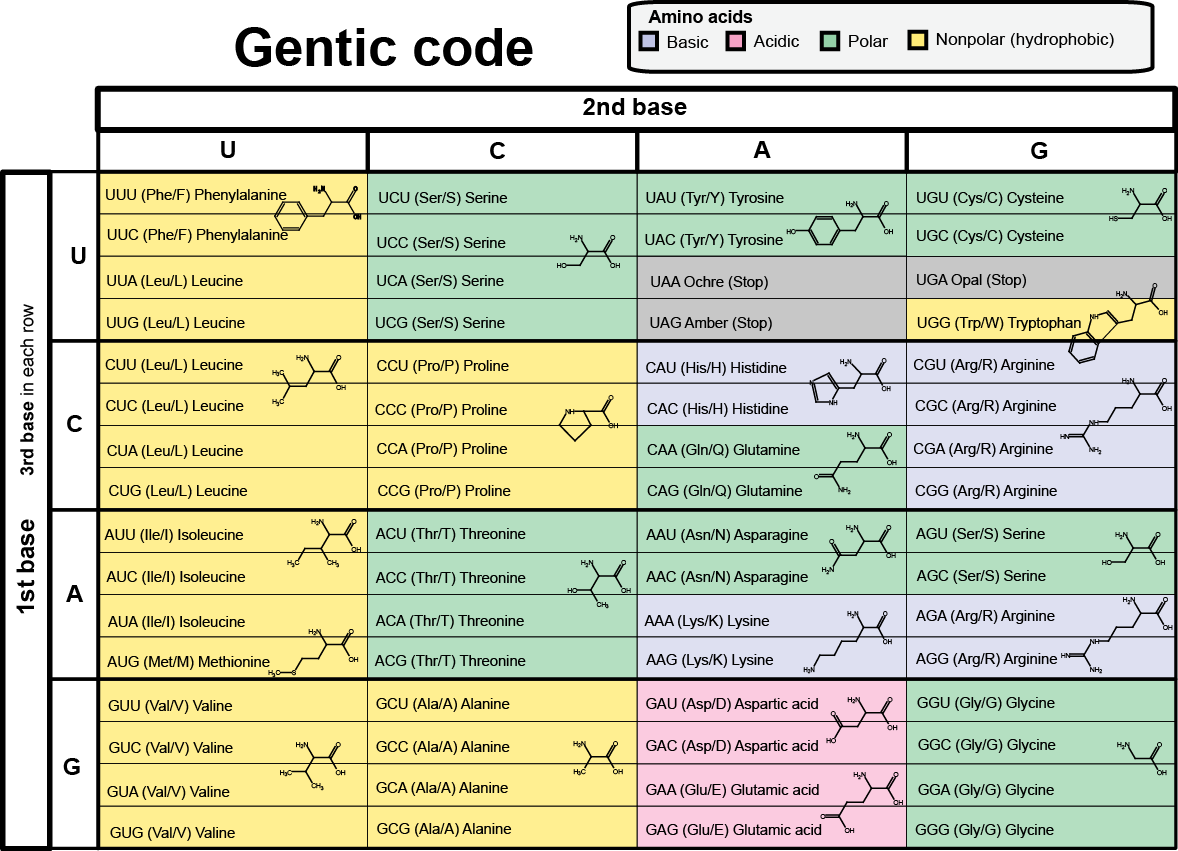
\includegraphics[width=0.7\textwidth]{fig01/genetic_code.png}
  \caption{Universal genetic code \newline (modified from the original version by \href{https://commons.wikimedia.org/wiki/File\%3ANotable_mutations.svg}{H\"aggstr\"om, Wikimedia Commons})}
\end{figure}

\noindent \textbf{Cellular functions of proteins}
\begin{itemize}
\item Enzymes: catalyze chemical reaction
\item Cell signaling: hormone (e.g. insulin), antibodies, …
\item Structural: collagen, cartilage, keratin, …
\end{itemize}

%
% Exercises 1.1
%
\subsubsection*{Exercises 1.1}
\begin{enumerate}

\item Draw a simple diagram of the central dogma of molecular biology and briefly explain the information flow of the molecules.

\item What are the DNA sequences of the opposite strand for the following DNA sequences?
\begin{verbatim}
    Seq1 CCGATT
    Seq2 TTACGC
    Seq3 ACGCGC
\end{verbatim}

\item What are the mRNA sequences transcribed from the following DNA sequences?

\item What are the polypeptide sequences translated from the following mRNA sequences? Answer them with both one-letter and three letter names.
\begin{verbatim}
    Seq1 AUGUUUUAA
    Seq2 GCAGCAAAA
\end{verbatim}
		
\end{enumerate}

%\end{document}

%\documentclass[12pt]{article}
%\usepackage[a4paper, margin=1in]{geometry} 
%\usepackage{graphicx} 
%\usepackage{hyperref}
%\usepackage{float}
%\usepackage[font=small, labelfont=bf]{caption}

%\begin{document}

%
% Introduction to Biotechnology
%
\subsection{Introduction to Biotechnology}
Biotechnology is the use of laboratory techniques to study living organism and cells. 

%
% Applications of biotechnology
%
\subsubsection*{Applications of biotechnology}
Branches of biotechnology can be explained with different colors.
\begin{itemize}
\item Red: medical processes
\item Green: agricultural processes
\item White: industrial processes
\item Blue: marine and aquatic applications
\end{itemize}

%
% Laboratory tools and equipment
%
\subsubsection*{Laboratory tools and equipment}

\begin{figure}[H]
  \centering
      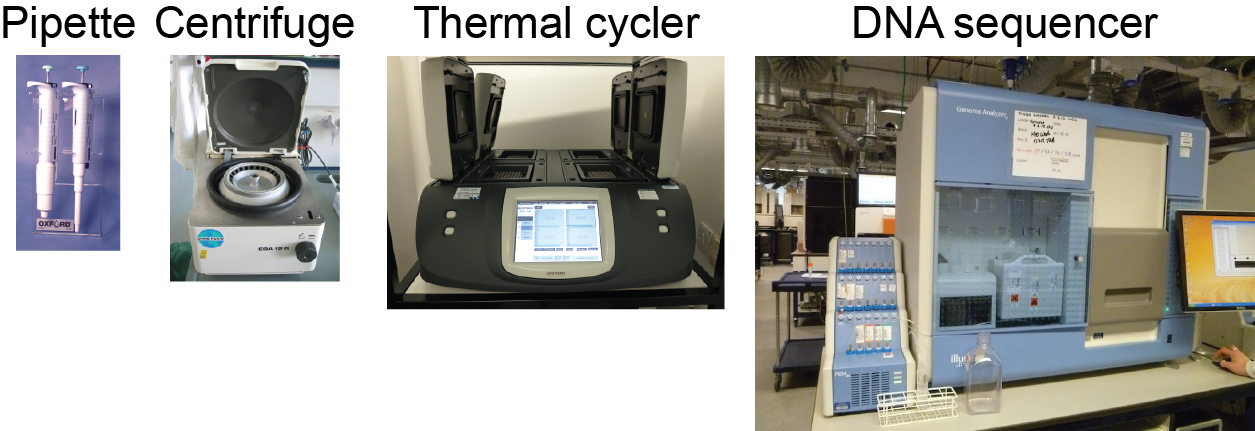
\includegraphics[width=0.5\textwidth]{fig01/lab_equipment.png}
  \caption{Pipette, centrifuge, thermal cycler, and DNA sequencer \newline (sources:  \href{https://en.wikipedia.org/wiki/Pipette\#/media/File:Single_channel_rack.jpg}{Domain}, \href{https://commons.wikimedia.org/w/index.php?curid=494}{Manske},
\href{https://commons.wikimedia.org/w/index.php?curid=20189025}{Rror}, 
\href{https://commons.wikimedia.org/w/index.php?curid=18862968}{RE73} via Wikimedia Commons)}
\end{figure}
 
%
% Human genome project
%
\subsubsection*{Human genome project}
It was a large-scale international research project to determine the whole DNA sequences of human.

\begin{itemize}
\item 1990 –- 2003
\item \$2.7 billion
\end{itemize}

%
% Next generation sequencing
%
\subsubsection*{Next generation sequencing}
Sequence technologies have been rapidly advanced since the human genome project.

Example: sequence a whole human genome with Illumina HiSeq X Ten.
\begin{itemize}
\item One day
\item \$1000
\end{itemize}

%
% Protein sequencing
%
\subsubsection*{Protein sequencing}
Proteins are generally more studied than DNAs and RNAs, but the whole proteome is generally harder to analyze than the whole genome. MS (mass-spectrometry) based technologies are widely used to sequence proteins.

\begin{figure}[H]
  \centering
      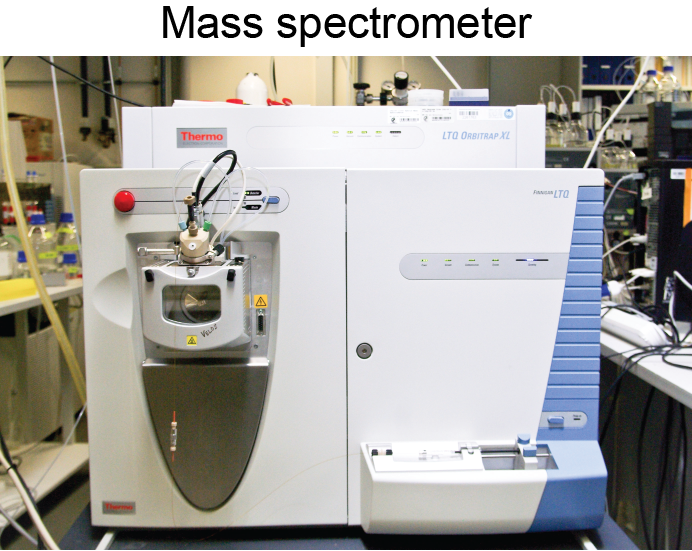
\includegraphics[width=0.25\textwidth]{fig01/mass_spectrometer.png}
  \caption{Orbitrap mass spectrometer (source: \href{https://commons.wikimedia.org/w/index.php?curid=18691799}{Wi\`{o}rkiewicz, Wikimedia Commons})}
\end{figure}
 
%\end{document}

%\documentclass[12pt]{article}
%\usepackage[a4paper, margin=1in]{geometry} 
%\usepackage{graphicx} 
%\usepackage{hyperref}
%\usepackage{float}
%\usepackage[font=small, labelfont=bf]{caption}
%
%\begin{document}

%
% Bioinformatics in INF281
%
\subsection{Bioinformatics in INF281}
Bioinformatics uses computational approaches to solve problems in life sciences. It is based on computer science.

%
% Similar or almost equivalent disciplines
%
\subsubsection*{Similar or almost equivalent disciplines}
\begin{itemize}
\item Biostatistics
\item Biophysics
\item Systems biology
\item Computational biology
\end{itemize}

%
% Not much related with bioinformatics
%
\subsubsection*{Not much related with bioinformatics}
\begin{itemize}
\item Health informatics
\item Forensic science
\end{itemize}

%
% Scope of INF281
%
\subsubsection*{Scope of INF281}
We mainly cover the following fields of bioinformatics in this course.
\begin{itemize}
\item Pairwise alignment
\item Database search
\item Statistical evaluation
\item Multiple alignment
\item Phylogenetic tree
\item Scoring scheme
\item Sequence patterns
\end{itemize}

%
% Popular bioinformatics programs
%
\subsubsection*{Popular bioinformatics programs}
BLAST and ClustalW are popular tools for sequence analysis.
\begin{itemize}
\item BLAST: a program for database search

URL: \url{http://blast.ncbi.nlm.nih.gov}

\item ClustalW: a program for multiple alignments

URL: \url{http://www.ch.embnet.org/software/ClustalW.html}

\end{itemize}

\begin{table}[!ht]
\scriptsize

\begin{tabular}{l p{10cm} r}
Rank & Title& Times cited \\
\hline
1 & Protein measurement with the folin phenol reagent & 305148 \\
2 & Cleavage of structural proteins during the assembly of the head of bacteriophage T4 & 213005 \\
3 & A rapid and sensitive method for the quantitation of microgram quantities of protein utilizing the principle of protein-dye binding & 155530 \\
4 & DNA sequencing with chain-terminating inhibitors & 65335 \\
5 & Single-step method of RNA isolation by acid guanidinium thiocyanate-phenol-chloroform extraction & 60397 \\
6 & Electrophoretic transfer of proteins from polyacrylamide gels to nitrocellulose sheets: procedure and some applications & 53349 \\
7 & Development of the Colle-Salvetti correlation-energy formula into a functional of the electron density & 46702 \\
8 & Density-functional thermochemistry. III. The role of exact exchange & 46145 \\
9 & A simple method for the isolation and purification of total lipides from animal tissues & 45131 \\
\textbf{10} & \textbf{Clustal W}: improving the sensitivity of progressive multiple sequence alignment through sequence weighting, position-specific gap penalties and weight matrix choice & 40289 \\
11 & Nonparametric estimation from incomplete observations & 38600 \\
\textbf{12} & \textbf{Basic local alignment search tool} & 38380 \\
13 & A short history of SHELX & 37978 \\
\textbf{14} & \textbf{Gapped BLAST and PSI-BLAST}: A new generation of protein database search programs & 36410 \\
15 & A revised medium for rapid growth and bio assays with tobacco tissue cultures & 36132 \\
\end{tabular}
\caption{The 15 most cited papers of all time \newline (The top 100 papers, Van Noorden, Maher, and Nuzzo, \textit{Nature}, 2014)}
\end{table}

%\end{document}


\newpage

%
% PART II
%
\part{}

%
% Global_pairwise_alignment
%
\setcounter{figure}{0}
\setcounter{table}{0}
\section{Global pairwise alignment}
%\documentclass[12pt]{article}
%\usepackage[a4paper, margin=1in]{geometry} 
%\usepackage{graphicx} 
%\usepackage{hyperref}
%\usepackage{float}
%\usepackage{multicol}
%\usepackage[font=small, labelfont=bf]{caption}
%
%\begin{document}

%
% Pairwise alignment
%
\subsection{Pairwise alignment}
A pairwise alignments is a basic sequence structure that consits of two sequences. A global alignment stretches to the whole part of two sequences, whereas a local alignment usually contains only part of the sequences.

%
% Pairwise alignment
%
\subsubsection*{Components of pairwise alignment}

We name two sequences as ‘database’ or ‘d’ and ‘query’ or ‘q’ through this course. They may represent sequences from two different species or organisms.
\\

\noindent
Identical sequences.
\begin{verbatim}
    q: ACGT
    d: ACGT
\end{verbatim}

\noindent
One mismatch.
\begin{verbatim}
    q: ACGT
    d: ACGA
\end{verbatim}

\noindent
The '-' symbol represents a blank. A single or a set of multile blanks further reprents a gap, which is an indication of insertion or deletion in the course of evoluation between two organisms.
\begin{verbatim}
    q: ACGT
    d: A-GT
\end{verbatim}

\noindent
\textbf{N.B.} A gap cannot be aligned with another gap.

%
% Example of a simple scoring scheme
%
\subsubsection*{Example of a simple scoring scheme}
\begin{itemize}
\item Match: 1
\item Mismatch: 0
\item Gap penalty: 1 (use -1 for the actual calculation)
\end{itemize}

\noindent
We may use the following notation.
\begin{itemize}
\item $R_{ab}$ = 1 for a = b
\item $R_{ab}$ = 0 for a $\neq$ b
\item g = 1
\end{itemize}

%
% NEW PAGE
%
\newpage 

%
% Exercise \thesection.1
%
\subsubsection*{Exercise \thesection.1}
Use the simple scoring scheme above and calculate the scores of the following two alignments.

\begin{multicols}{2}
\begin{verbatim}
Alignment 1
    q: GCA-GCA
    d: GA-TG-A	
\end{verbatim}

\begin{verbatim}
Alignment 2 
    q: GCA-GCA
    d: GA-TG-A	
\end{verbatim}
\end{multicols}

%\end{document}

%\documentclass[12pt]{article}
%\usepackage[a4paper, margin=1in]{geometry} 
%\usepackage{graphicx} 
%\usepackage{hyperref}
%\usepackage{float}
%\usepackage{multicol}
%\usepackage[font=small, labelfont=bf]{caption}
%
%\begin{document}

%
% Alignment by brute-force
%
\subsection{Alignment by brute--force}
A brute--force approach finds the alignment with the highest score by simply considering all possible alignments and calculates the score for each of them.

%
% An example of brute--force approach
%
\subsubsection*{An example of brute--force approach}
We find the optimal alignment for the following sequences by using the scoring scheme below.

\begin{multicols}{2}
Sequences:
\begin{verbatim}
    q: AG, d: ACG
\end{verbatim}
\vfill\null
\columnbreak

\noindent Scoring scheme: \\ 
\null \quad $R_{ab}$ = 1 for a = b \\ 
\null \quad $R_{ab}$ = 0 for a $\neq$ b \\ 
\null \quad g = 1

\end{multicols} 

\noindent \textbf{1. The length of alignment}
\begin{itemize}
\item Maximum length: length(q) + length(d)
\item Minimum length: max(length(q), length(d))
\end{itemize}
\medskip 

\noindent \textbf{2. All possible alignments when length = 5}
\begin{verbatim}
    ---AG    A---G    A--G-    AG---    --A-G
    ACG--    -ACG-    -AC-G    --ACG    AC-G-

    --AG-    -AG--    -A--G    -A-G-    A-G--
    AC--G    A--CG    A-CG-    A-C-G    -A-CG
\end{verbatim}
\medskip

\noindent \textbf{3. All possible alignments when length = 4}
\begin{verbatim}
    A--G    A-G-    AG--    A--G    -A-G    -AG-
    ACG-    AC-G    A-CG    -ACG    ACG-    AC-G

    -AG-    A-G-    --AG    --AG    -A-G    AG--
    A-CG    -ACG    ACG-    AC-G    A-CG    -ACG
\end{verbatim}
\medskip

\noindent \textbf{4. All possible alignments when length = 3}
\begin{verbatim}
    -AG    A-G    AG-
    ACG    ACG    ACG
\end{verbatim}
\medskip

\noindent \textbf{5. Alignment with the best score}
\begin{verbatim}
    ACG
    A-G	
\end{verbatim}

Score: 1

%
% Search space size of the brute-force approach
%
\subsubsection*{Search space size of the brute-force approach}
The search space size is the number of all possible alignments. It is 25 (10 + 12 + 3) for the example above. \\

\noindent \textbf{Rapid growth of search space size}

\begin{multicols}{2}
\begin{verbatim}
Example 1
    q: ACGACG, d: AGAG
\end{verbatim}
Search space size: 1289

\begin{verbatim}
Example 2
    q: ACGACGACGACG, d: AGAGAGAG
\end{verbatim}
Search space size: 4,673,345

\end{multicols}

%
% Exercise \thesection.2
%
\subsubsection*{Exercise \thesection.2}
Find the alignment with the best score for the sequences.  Use the simple scoring scheme below.

\begin{multicols}{2}
Sequences:
\begin{verbatim}
    q: A, d: AC
\end{verbatim}
\vfill\null
\columnbreak

\noindent Scoring scheme: \\ 
\null \quad $R_{ab}$ = 1 for a = b \\ 
\null \quad $R_{ab}$ = 0 for a $\neq$ b \\ 
\null \quad g = 1

\end{multicols} 

\begin{enumerate}
\item What are the maximum and minimum lengths of the alignment?
\item Identify all possible alignments.
\item What is the best score?
\item What is the search space size when the brute-force approach is used?
\end{enumerate}

%\end{document}

%\documentclass[12pt]{article}
%\usepackage[a4paper, margin=1in]{geometry} 
%\usepackage{graphicx} 
%\usepackage{hyperref}
%\usepackage{float}
%\usepackage{multicol}
%\usepackage[font=small, labelfont=bf]{caption}
%
%\begin{document}

%
% Alignment by brute-force
%
\subsection{Table representation of alignment}
Several data strcutres can be used to repesent an alignment. The table representation is frequently used and also makes the process clear when we combine it with dynamic programming (DP) later.

\subsubsection*{Data structures and algorithms}
It is important to consider the following aspects before solving computational problems.
\begin{enumerate}
\item Identify and analyze the problem you want to solve
\item Pick up an algorithm that can efficiently solve the problem
\item Decide a data structure that works with the algorithm of your choice
\end{enumerate}

\noindent We use a table format (2D array) to solve global alignments by dynamic programming.

\subsubsection*{Example of table format}
Alignment:
\begin{verbatim}
    q: -AG-
    d: A-CG
\end{verbatim}
\medskip 

\noindent \textbf{1. Initial setup}

\begin{enumerate}
\item Make a table with the size of (1 + length(q)) by (1 + length(b))
\item Add the database sequence as column labels
\item And the query sequence as row labels
\end{enumerate}

\begin{figure}[H]
  \centering
      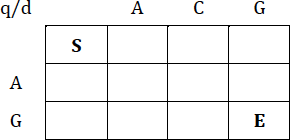
\includegraphics[width=0.3\textwidth]{fig02/alignment_to_table.png}
\end{figure}

\noindent \textbf{2. Add arrows}

We use three types of arrows to form an alignment.
\begin{itemize}
\item Move diagonally: add the letters from ‘q’ and ‘d’ to the alignment
\item Move vertically: add ‘-’ and the letter from ‘d’ to the alignment
\item Move horizontally: add the letter from ‘q’ and ‘-’ to the alignment
\end{itemize}

It shoud start from S and stops at E.

\begin{figure}[H]
  \centering
      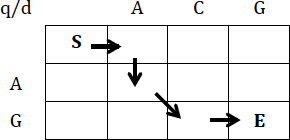
\includegraphics[width=0.3\textwidth]{fig02/alignment_to_table_example.png}
\end{figure}

%
% Exercise \thesection.3
%
\subsubsection*{Exercise \thesection.3}

Find the corresponding alignments for Table 1, 2 and 3.

\begin{multicols}{3}
Table 1
\begin{figure}[H]
  \centering
      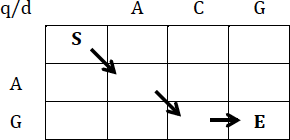
\includegraphics[width=0.3\textwidth]{fig02/alignment_to_table_exercise1.png}
\end{figure}

Table 2
\begin{figure}[H]
  \centering
      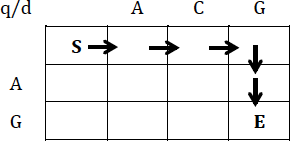
\includegraphics[width=0.3\textwidth]{fig02/alignment_to_table_exercise2.png}
\end{figure}

Table 3
\begin{figure}[H]
  \centering
      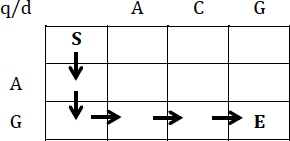
\includegraphics[width=0.3\textwidth]{fig02/alignment_to_table_exercise3.png}
\end{figure}

\end{multicols} 

%\end{document}

%\documentclass[12pt]{article}
%\usepackage[a4paper, margin=1in]{geometry} 
%\usepackage{graphicx} 
%\usepackage{hyperref}
%\usepackage{float}
%\usepackage{multicol}
%\usepackage{amsmath}
%\usepackage[ruled]{algorithm2e}
%\usepackage[font=small, labelfont=bf]{caption}
%
%\begin{document}

%
% Global alignment with DP
%
\subsection{Global alignment with DP}
Dynamic programming (DP) provides a solution for a multi-stage decision process, in which larger decisions recursively nest smaller decisions.

\subsubsection*{Memorize the best score in a table cell}

The most basic step of DP procedures is updatig a cell with the hightet score from the three different scores calculated from its adjacent cells. DP ends when all the table cells are updated.

\begin{figure}[H]
  \centering
      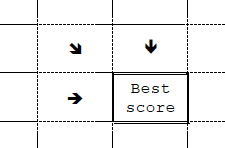
\includegraphics[width=0.25\textwidth]{fig02/dynamic_programmoing_cell_update.png}
\end{figure}

%
% Table notation and indices
%	
\subsubsection*{Table notation and indices}
$H_{i,j}$ represents the score of the cell for the current update. $H_{i-1,j}$, $H_{i,j-1}$,and $H_{i-1,j-1}$ are the scores of the adjacent cells.

\begin{multicols}{2}

Cell $H_{i, j}$ and its adjcent cells
\begin{figure}[H]
  \centering
      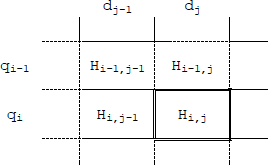
\includegraphics[width=0.3\textwidth]{fig02/dynamic_programmoing_cell_indices.png}
\end{figure}

Example
\begin{figure}[H]
  \centering
      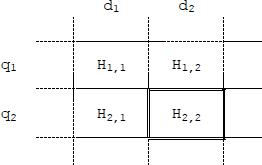
\includegraphics[width=0.3\textwidth]{fig02/dynamic_programmoing_cell_indices_example.png}
\end{figure}

\end{multicols} 

%
% Calculation of three candidate scores
%	
\subsubsection*{Calculation of three candidate scores}
$H_{i,j}^{(0)}$, $H_{i,j}^{(1)}$, and $H_{i,j}^{(2)}$ represent the three candidate scores of $H_{i,j}$. They are respectively calculated as:
\begin{align*}
H_{i,j}^{(0)} &= H_{i-1,j} - g &(vertical) \\
H_{i,j}^{(1)} &= H_{i,j-1} - g	&(horizontal) \\
H_{i,j}^{(2)} &= H_{i-1,j-1} + R_{a,b} &(diagonal)
\end{align*}

%
% Exercise \thesection.4
%
\subsubsection*{Exercise \thesection.4}

Calculate the scores of $H_{4,6}^{(0)}$, $H_{4,6}^{(1)}$, and $H_{4,6}^{(2)}$ first and then update $H_{4,6}$.
\begin{multicols}{2}
\begin{figure}[H]
  \centering
      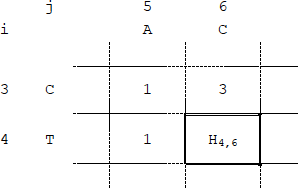
\includegraphics[width=0.3\textwidth]{fig02/dynamic_programmoing_cell_update_exercise.png}
\end{figure}

\noindent Scoring scheme: \\ 
$R_{ab}$ = 1 for a = b \\ 
$R_{ab}$ = 0 for a $\neq$ b \\ 
g = 1

\end{multicols} 

%
% Initialization
%
\subsubsection*{Initialization}

The first row and the first column can be calcuated independently from the adjcent cells.
\begin{align*}
H_{0,j} &:  j * -1 * g \\
H_{i,0} &: i * -1 * g
\end{align*}

\noindent
Example
\begin{figure}[H]
  \centering
      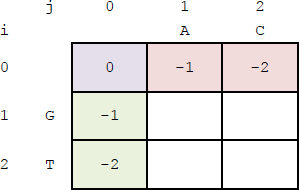
\includegraphics[width=0.3\textwidth]{fig02/dynamic_programmoing_initialization.png}
\end{figure}

%
% Exercise \thesection.5
%
\subsubsection*{Exercise \thesection.5}
Update all cells of Table 1 and 2. Use the scoring scheme in Exercise \thesection.4.

\begin{multicols}{2}
Table 1
\begin{figure}[H]
  \centering
      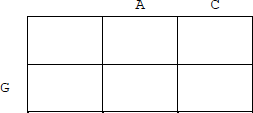
\includegraphics[width=0.3\textwidth]{fig02/global_alignment_exercise1.png}
\end{figure}

\vfill\null
\columnbreak

Table 2
\begin{figure}[H]
  \centering
      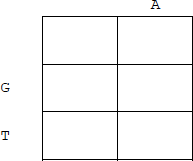
\includegraphics[width=0.25\textwidth]{fig02/global_alignment_exercise2.png}
\end{figure}

\end{multicols} 

%
% Sub-solutions
%
\subsubsection*{Sub-solutions}

In DP, larger decisions recursively nest smaller decisions. For instance, Table S is included in Table L.

\begin{multicols}{2}
Table S
\begin{figure}[H]
  \centering
      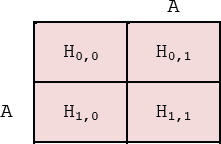
\includegraphics[width=0.3\textwidth]{fig02/dynamic_programmoing_subsolution_S.png}
\end{figure}

\vfill\null
\columnbreak

Table L
\begin{figure}[H]
  \centering
      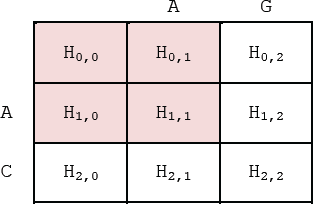
\includegraphics[width=0.4\textwidth]{fig02/dynamic_programmoing_subsolution_L.png}
\end{figure}

\end{multicols} 

%
% NEW PAGE
%
\newpage

%
% Psedo-code of global alignment with DP
%
\subsubsection*{Psedo-code of updating DP table for global alignment}

\begin{algorithm}[H]
  \SetKwInOut{HAB}{$\mathrm{H_{i,j}}$}
  \SetKwInOut{RAB}{$\mathrm{R_{a,b}}$}
  \SetKwInOut{G}{$\mathrm{g}$}
  \SetKwData{dRAB}{$\mathrm{R_{a,b}}$}
  \SetKwData{dG}{$\mathrm{g}$}
  
  \BlankLine
    
  \HAB{Dyanamic programming table}
  \RAB{Match/mismatch scores}
  \G{Gap penalty}
  
  \BlankLine \BlankLine
  
  \tcp{Initialization}
  \For{$i \leftarrow 0$ \KwTo $m$}{
    $\mathrm{H_{i,0}}$ $\leftarrow$ $i * -1 * g$\;
  }
  \For{$j \leftarrow 1$ \KwTo $n$}{
    $\mathrm{H_{0,j}}$ $\leftarrow$ $j * - 1 * g$\;
  }
  
  \BlankLine \BlankLine
    
  \tcp{Main loop for table update}
  \For{$i \leftarrow 1$ \KwTo $m$}{
    \For{$j \leftarrow 1$ \KwTo $n$}{
      $\mathrm{H_{i,j}}$ $\leftarrow$ $max(\mathrm{H_{i-1,j}} - \dG, \mathrm{H_{i,j-1}} - \dG, \mathrm{H_{i-1,j-1}}$ + \dRAB)\;
    }
  }
  
  \SetAlgoRefName{\thesection.1}
  \caption{Update dynamic programming table for global alignment}

\end{algorithm}

%\end{document}

%\documentclass[12pt]{article}
%\usepackage[a4paper, margin=1in]{geometry} 
%\usepackage{graphicx} 
%\usepackage{hyperref}
%\usepackage{float}
%\usepackage{multicol}
%\usepackage{amsmath}
%\usepackage[ruled]{algorithm2e}
%\usepackage{amssymb}
%\usepackage[font=small, labelfont=bf]{caption}

%\begin{document}

%
% Backtracking
%
\subsection{Backtracking}
Backtracking is a post-processing procedure to find the alignments that have yielded the best score. 

%
% Store movement in cells
%
\subsubsection*{Store movement in cells}

A table cell can be used for storing the movement.
\begin{figure}[H]
  \centering
      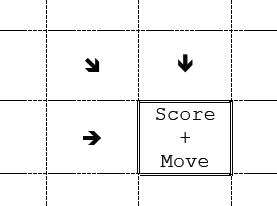
\includegraphics[width=0.3\textwidth]{fig02/back_tracking_store_moves.png}
\end{figure}

\noindent \textbf{Example}
\begin{multicols}{2}
Cells with scores and directions
\begin{figure}[H]
  \centering
      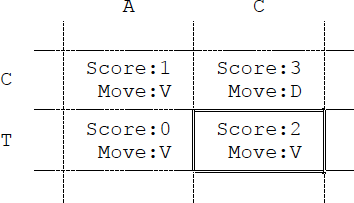
\includegraphics[width=0.3\textwidth]{fig02/back_tracking_store_moves_example.png}
\end{figure}

Use arrows to indicate backtracking
\begin{figure}[H]
  \centering
      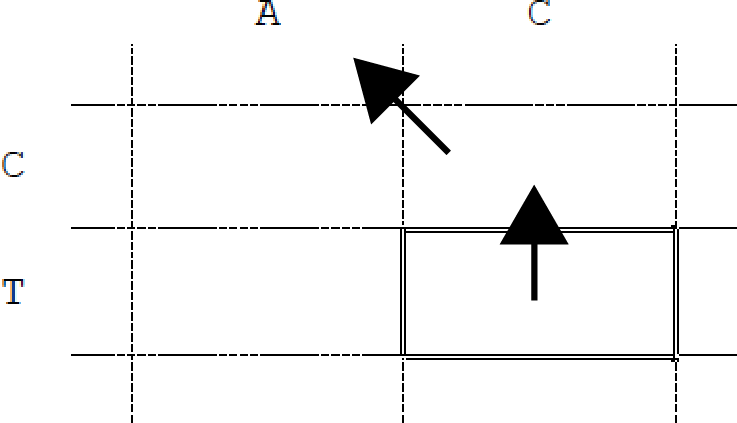
\includegraphics[width=0.3\textwidth]{fig02/back_tracking_store_moves_arrows.png}
\end{figure}

\end{multicols} 

%
% Exercise \thesection.6
%
\subsubsection*{Exercise \thesection.6}
	
Complete the DP table with scores and directions. What is the alignment with the best score?

\begin{multicols}{2}
\begin{figure}[H]
  \centering
      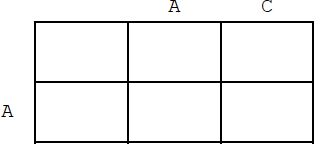
\includegraphics[width=0.3\textwidth]{fig02/back_tracking_store_moves_exercise.png}
\end{figure}

\noindent Scoring scheme: \\ 
$R_{ab}$ = 1 for a = b \\ 
$R_{ab}$ = 0 for a $\neq$ b \\ 
g = 1

\end{multicols} 

%
% Re-calculate candidate scores
%
\subsubsection*{Re-calculate candidate scores}

Re-calculating the three candidate scores also reveals the movement.

\begin{align*}
H_{i,j}^{(0)} &= H_{i-1,j} - g &(vertical) \\
H_{i,j}^{(1)} &= H_{i,j-1} - g &(horizontal) \\
H_{i,j}^{(2)} &= H_{i-1,j-1} + R_{a,b} &(diagonal)
\end{align*}

\noindent \textbf{Example}

\begin{figure}[H]
  \centering
      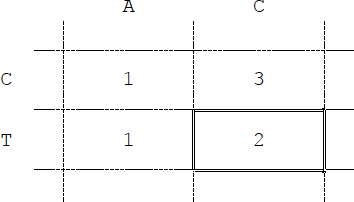
\includegraphics[width=0.3\textwidth]{fig02/back_tracking_example.png}
\end{figure}
				
\begin{align*}
H_{i,j}^{(0)} &= 3 - 1 = 2 = H_{i,j} &\checkmark & (vertical) \\
H_{i,j}^{(1)} &= 1 - 1 = 0 \neq H_{i,j} &\hfill & (horizontal) \\
H_{i,j}^{(2)} &= 1 + 0 = 1 \neq H_{i,j} &\hfill  & (diagonal)
\end{align*}

%
% Common mistake with backtracking
%
\subsubsection*{Common mistake with backtracking}
For the re-calculation approach, it is not to find $max(H_{i-1,j}, H_{i,j-1}, H_{i-1,j-1})$. You must re-calculate the candidates and then $max(H_{i,j}^{(0)}, H_{i,j}^{(1)} , H_{i,j}^{(2)})$ to find the actual direction.

%
% Implementation with recursive call
%
\subsubsection*{Implementation with recursive call}
Recursive calls are usually used to implement DP backtracking.

\begin{algorithm}[H]
  \SetKwInOut{HAB}{$\mathrm{H_{i,j}}$}
  \SetKwInOut{RAB}{$\mathrm{R_{a,b}}$}
  \SetKwInOut{G}{$\mathrm{g}$}
  
  \SetKwProg{Fn}{proc}{}{end}
  \SetKwInOut{I}{$\mathrm{i}$}
  \SetKwInOut{J}{$\mathrm{j}$}
  \SetKwInOut{SQ}{$\mathrm{S_{q}}$}
  \SetKwInOut{SD}{$\mathrm{S_{d}}$}
  \SetKwInOut{AQ}{$\mathrm{A_{q}}$}
  \SetKwInOut{AD}{$\mathrm{A_{d}}$}
  \SetKwInOut{K}{$\mathrm{k}$}

  \SetKwData{dI}{$\mathrm{i}$}
  \SetKwData{dJ}{$\mathrm{j}$}
  \SetKwData{dAQ}{$\mathrm{A_{q}}$}
  \SetKwData{dAD}{$\mathrm{A_{d}}$}
  \SetKwData{dK}{$\mathrm{k}$}
    
  \SetKwData{dRAB}{$\mathrm{R_{a,b}}$}
  \SetKwData{dG}{$\mathrm{g}$}

  \BlankLine
  
  \SQ{Sequence q}
  \SD{Sequence d}     
  \HAB{Dynamic programming table}
  \RAB{Match/mismatch scores}
  \G{Gap penalty}

  \BlankLine \BlankLine

  \Fn{backTrack(\dI, \dJ, \dAQ, \dAD, \dK)}{
    
    \BlankLine
    
    \I{Index of sequence q}
    \J{Index of sequence d}
    \AQ{q part of alignment (stored in reverse order)}
    \AD{d part of alignment (stored in reverse order)}
    \K{Index for \dAQ and \dAD}
  
    \BlankLine
    
    \tcp{}
    \tcp{Need to implement recursion termination here}
    \tcp{...}
    \tcp{}
        
    \BlankLine
    
    \If(\tcp*[f]{vertical}){$\mathrm{H_{i,j}} = \mathrm{H_{i-1,j}} - g$}{
      $\mathrm{A_{q, k}} $ $\leftarrow$ $ S_{q, i}$\;
      $\mathrm{A_{d, k}} $ $\leftarrow$ $ $ '-'\;
      $backTrack$($\mathrm{i-1}$, \dJ, \dAQ, \dAD, $k + 1$)\;
    }
    \BlankLine

    \If(\tcp*[f]{horizontal}){$\mathrm{H_{i,j}} = \mathrm{H_{i,j-1}} - g$}{
      $\mathrm{A_{q, k}} $ $\leftarrow$ '-'\;
      $\mathrm{A_{d, k}} $ $\leftarrow$ $ S_{d, i}$\;
      $backTrack$(\dI, $\mathrm{j-1}$, \dAQ, \dAD, $k + 1$)\;
    }
    \BlankLine
    
    \If(\tcp*[f]{diagonal}){$\mathrm{H_{i,j}} = \mathrm{H_{i-1,j-1}} +\mathrm{R_{S_{q, i},S_{d, i}}}$}{
      $\mathrm{A_{q, k}} $ $\leftarrow$ $ S_{q, i}$\;
      $\mathrm{A_{d, k}} $ $\leftarrow$ $ S_{d, i}$\;
      $backTrack$($\mathrm{i-1}$, $\mathrm{j-1}$, \dAQ, \dAD, $k + 1$)\;
    }
      
    \BlankLine
  }

  \SetAlgoRefName{\thesection.2}
  \caption{DP backtracking}

\end{algorithm}

%
% Exercise \thesection.7
%
\subsubsection*{Exercise \thesection.7}
	
Find the alignment with the best score.

\begin{multicols}{2}
\begin{figure}[H]
  \centering
      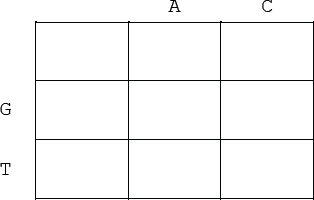
\includegraphics[width=0.3\textwidth]{fig02/back_tracking_exercise.png}
\end{figure}

\noindent Scoring scheme: \\ 
$R_{ab}$ = 1 for a = b \\ 
$R_{ab}$ = 0 for a $\neq$ b \\ 
g = 1

\end{multicols} 

%\end{document}

%\documentclass[12pt]{article}
%\usepackage[a4paper, margin=1in]{geometry} 
%\usepackage{graphicx} 
%\usepackage{hyperref}
%\usepackage{float}
%\usepackage{multicol}
%\usepackage{amsmath}
%\usepackage[ruled]{algorithm2e}
%\usepackage{amssymb}
%\usepackage[font=small, labelfont=bf]{caption}
%
%\begin{document}

%
% Needleman-Wunsch
%
\subsection{Needleman-Wunsch algorithm}
The method of using DP to solve global pairwise alignment is called the Needleman-Wunsch algorithm in the field of bioinformatics. 

%
% Complexity
%
\subsubsection*{Complexity}
\begin{itemize}
\item Time: O(nm)
\item Space: O(nm)
\end{itemize}

%
% Comparisons with other algorithms
%
\subsubsection*{Comparisons with other algorithms}
The Needleman-Wunsch algorithm is similar to several algorithms.
\\

\noindent
\textbf{Divide and conquer algorithms}

\noindent
Sub-solutions must be independent with divide and conquer.

\begin{figure}[H]
  \centering
      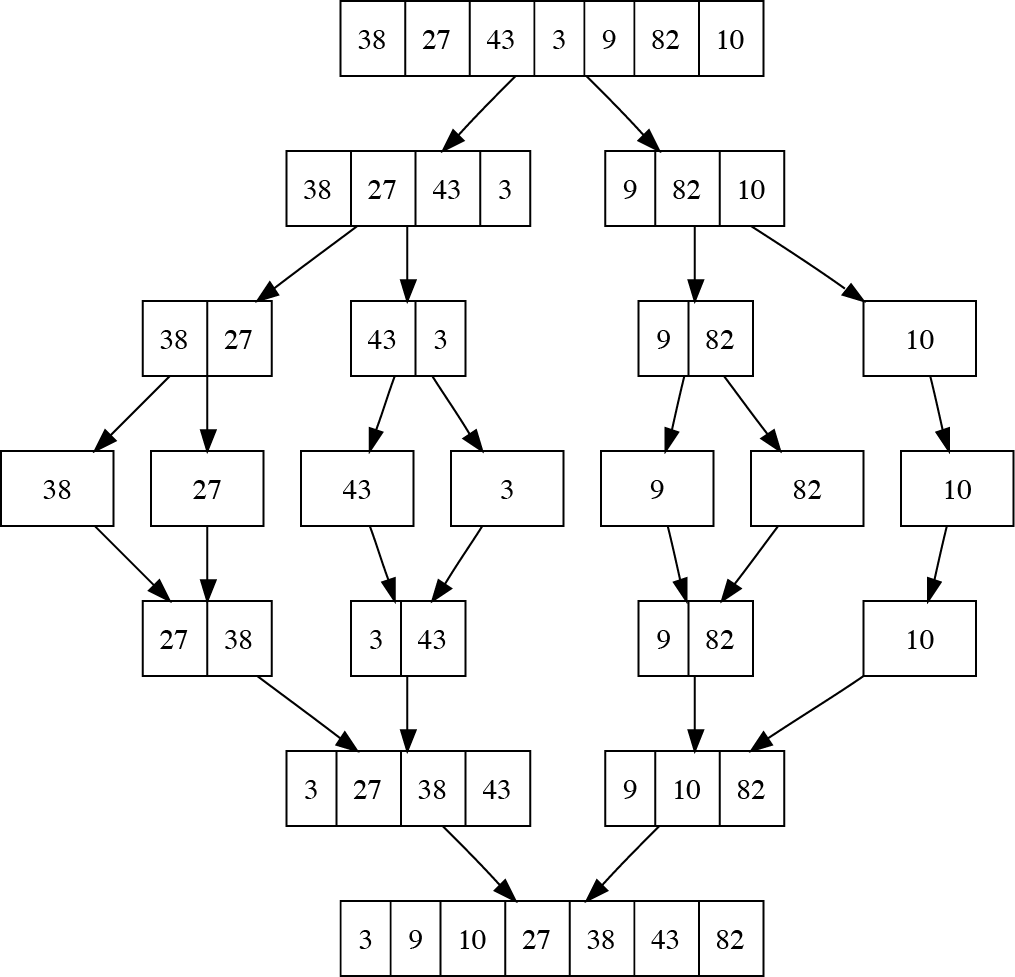
\includegraphics[width=0.25\textwidth]{fig02/Merge_sort_algorithm.png}
  \caption{Merge sort (source: \href{https://commons.wikimedia.org/w/index.php?curid=8004317}{VineetKumar, Wikimedia Commons})}
\end{figure}

\noindent
\textbf{Dijkstra's algorithm}

\noindent
Worst-case performance of Dijkstra: $O(|E|+|V|\log |V|)$

\begin{figure}[H]
  \centering
      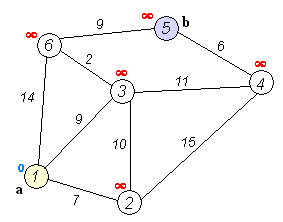
\includegraphics[width=0.25\textwidth]{fig02/Dijkstra.png}
  \caption{Dijkstra's algorithm (source: \href{https://commons.wikimedia.org/w/index.php?curid=6282617}{Ibmua, Wikimedia Commons})}
\end{figure}

%\end{document}


\newpage

%
% Extension_of_global_alignment
%
\setcounter{figure}{0}
\setcounter{table}{0}
\section{Extension of global alignment}
%\documentclass[12pt]{article}
%\usepackage[a4paper, margin=1in]{geometry} 
%\usepackage{graphicx} 
%\usepackage{hyperref}
%\usepackage{float}
%\usepackage{multicol}
%\usepackage[font=small, labelfont=bf]{caption}
%
%\begin{document}

%
% Homology at the sequence level
%
\subsection{Homology at the sequence level}
Constructing alignments can be useful to understand homology among different species. Finding homologies is important to reveal a common evolutionary ancestor.

%
% Evolution and homology
%
\subsubsection*{Evolution and homology}
All species are derived from a common ancestor at some point during the course of evolution.
 
\begin{figure}[H]
  \centering
      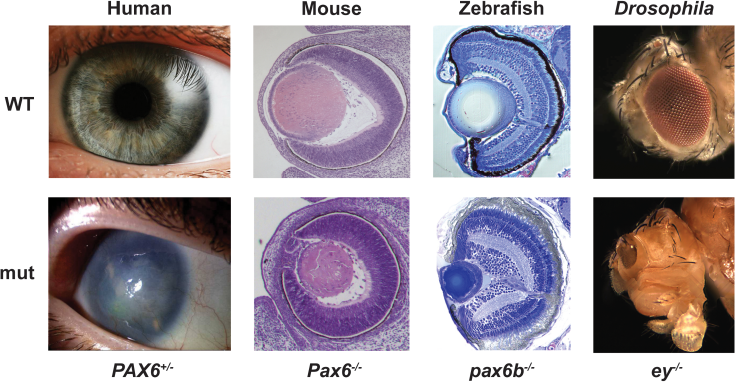
\includegraphics[width=0.5\textwidth]{fig03/PAX6_mutation.png}
  \caption{PAX6 alterations result in similar changes to eye morphology \newline (source: Washington et al, doi: 10.1371/journal.pbio.1000247 via \href{https://commons.wikimedia.org/w/index.php?curid=8626896}{Wikimedia Commons})}
\end{figure}

%
% Homologous and  analogous
%
\subsubsection*{Homologous and  analogous}
It is useful to check similarity at the molecular level because there are cases that analogous structures may not indicate homologous. 
\begin{figure}[H]
  \centering
      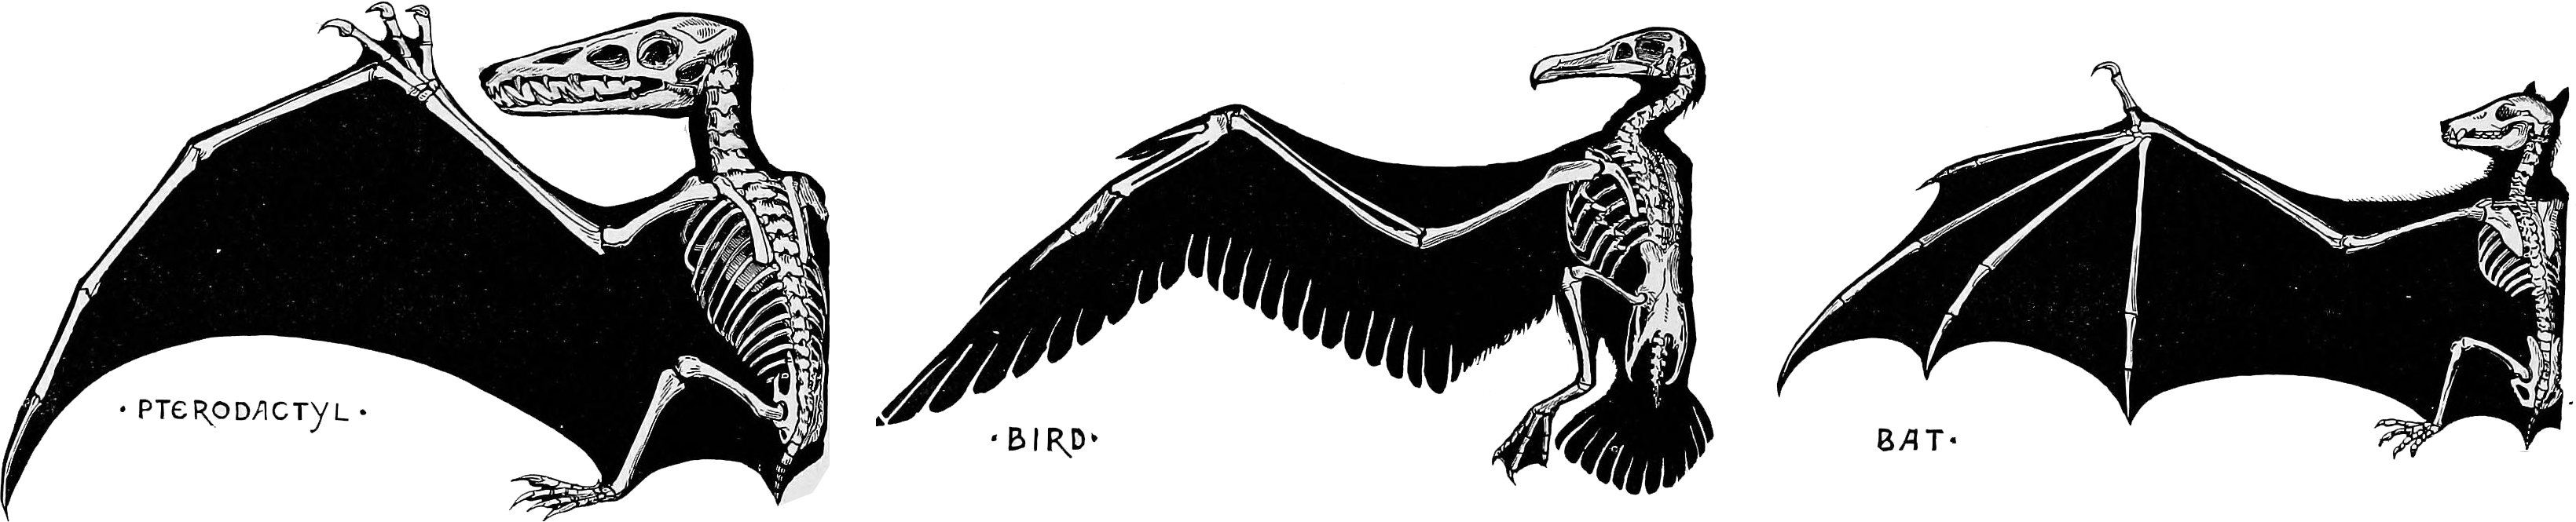
\includegraphics[width=0.5\textwidth]{fig03/analogous.png}
  \caption{Homologous and  analogous structures \newline (source: John Romanes, 1892, Darwin and after Darwin via \href{https://commons.wikimedia.org/w/index.php?curid=1324636}{Wikimedia Commons})}
\end{figure}

%
% Sequence homology
%
\subsubsection*{Sequence homology}
\begin{figure}[H]
  \centering
      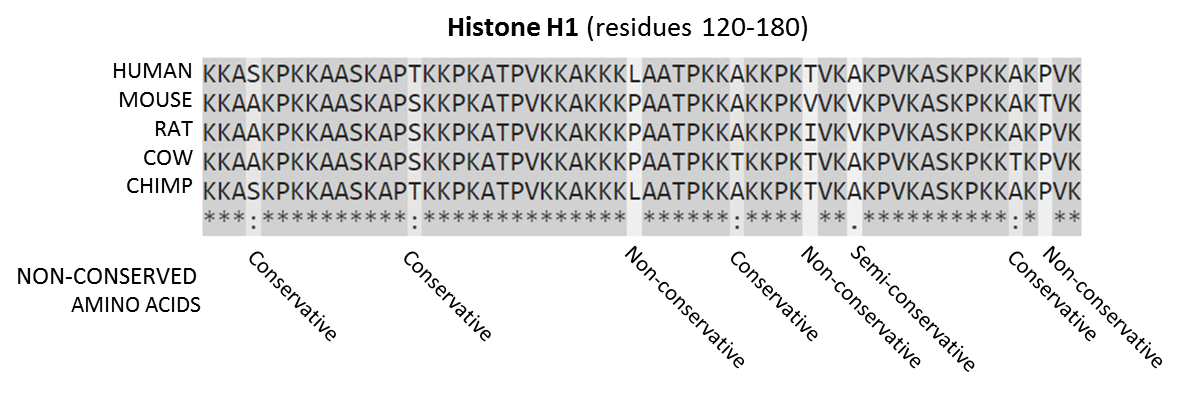
\includegraphics[width=0.75\textwidth]{fig03/histone_alignment.png}
  \caption{Multiple sequence alignment of histon sequences \newline (source: \href{https://commons.wikimedia.org/w/index.php?curid=37188728}{Shafee, Wikimedia Commons})}
\end{figure}

%
% Sequence homology
%
\subsubsection*{Evolution at the sequence level}
Sequence differences in DNA
\begin{itemize}
\item Substitution (a mismatch in alignment)
\item Insertion (a gap in alignment)
\item Deletion (a gap in alignment)
\item Inversion
\end{itemize}

\noindent
Source of variations
\begin{itemize}
\item Mutation
\item Recombination
\item Insertional mutagenesis
\item ...
\end{itemize}

\noindent
A mutation of the third nucleotide in a codon often does not affect which amino acid is synthesized.
\begin{itemize}
\item GCU $\rightarrow$ Ala (Alanine)
\item GCC $\rightarrow$ Ala (Alanine)
\item GCA $\rightarrow$ Ala (Alanine)
\item GCG $\rightarrow$ Ala (Alanine)
\end{itemize}

\noindent
An amino acid can be replaced by a different amino acid that has similar properties in some cases.
\begin{itemize}
\item AUU, AUC, AUA $\rightarrow$ Ile (Isoleucine)
\item CUU, CUC, CUA $\rightarrow$ Leu (Leucine)
\end{itemize}

%
% Extension of global alignment
%
\subsubsection*{Extension of global alignment with DP}

\begin{itemize}
\item Score matrix \\
DNA, RNA, and protein

\item Gap penatlty \\
Linear, affine, and constant
\end{itemize}



%\end{document}

%\documentclass[12pt]{article}
%\usepackage[a4paper, margin=1in]{geometry} 
%\usepackage{graphicx} 
%\usepackage{hyperref}
%\usepackage{float}
%\usepackage{multicol}
%\usepackage[font=small, labelfont=bf]{caption}
%
%\begin{document}

%
% Introduction of score matrix
%
\subsection{Introduction of score matrix}
We will expand our simple scoring scheme to score matrices. This expansion allows us to solve general alignment problems with DNA, RNA, and protein sequences. 

%
% Extension of a scoring scheme to a score matrix
%
\subsubsection*{Extension of a scoring scheme to a score matrix}
The matrix below is equivalent with match: 1 and mismatch: 0. 

\begin{figure}[H]
  \centering
      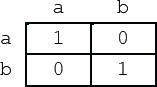
\includegraphics[width=0.175\textwidth]{fig03/simple_score_matrix.png}
\end{figure}

\noindent
\textbf{Example of a DNA score matrix}

\noindent
The matrix below is equivalent with match: 5 and mismatch: -4. 

\begin{figure}[H]
  \centering
      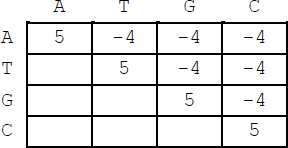
\includegraphics[width=0.3\textwidth]{fig03/dna_matrix_exercise.png}
\end{figure}

%
% Applications of score matrix
%
\subsubsection*{Applications of score matrix}

Score matrices are more flexible than the simple scoring scheme. For instance, they can be used for the following cases.

\begin{itemize}
\item DNA pairs
\item RNA pairs
\item Similarity of protein sequences by amino acid properties
\end{itemize}

%
% DNA pairs (Watson-Crick pairs)
%
\subsubsection*{DNA pairs (Watson-Crick pairs)}
A thymine pairs with an adenine, and a cytosine pairs with a guanine.

\begin{figure}[H]
  \centering
      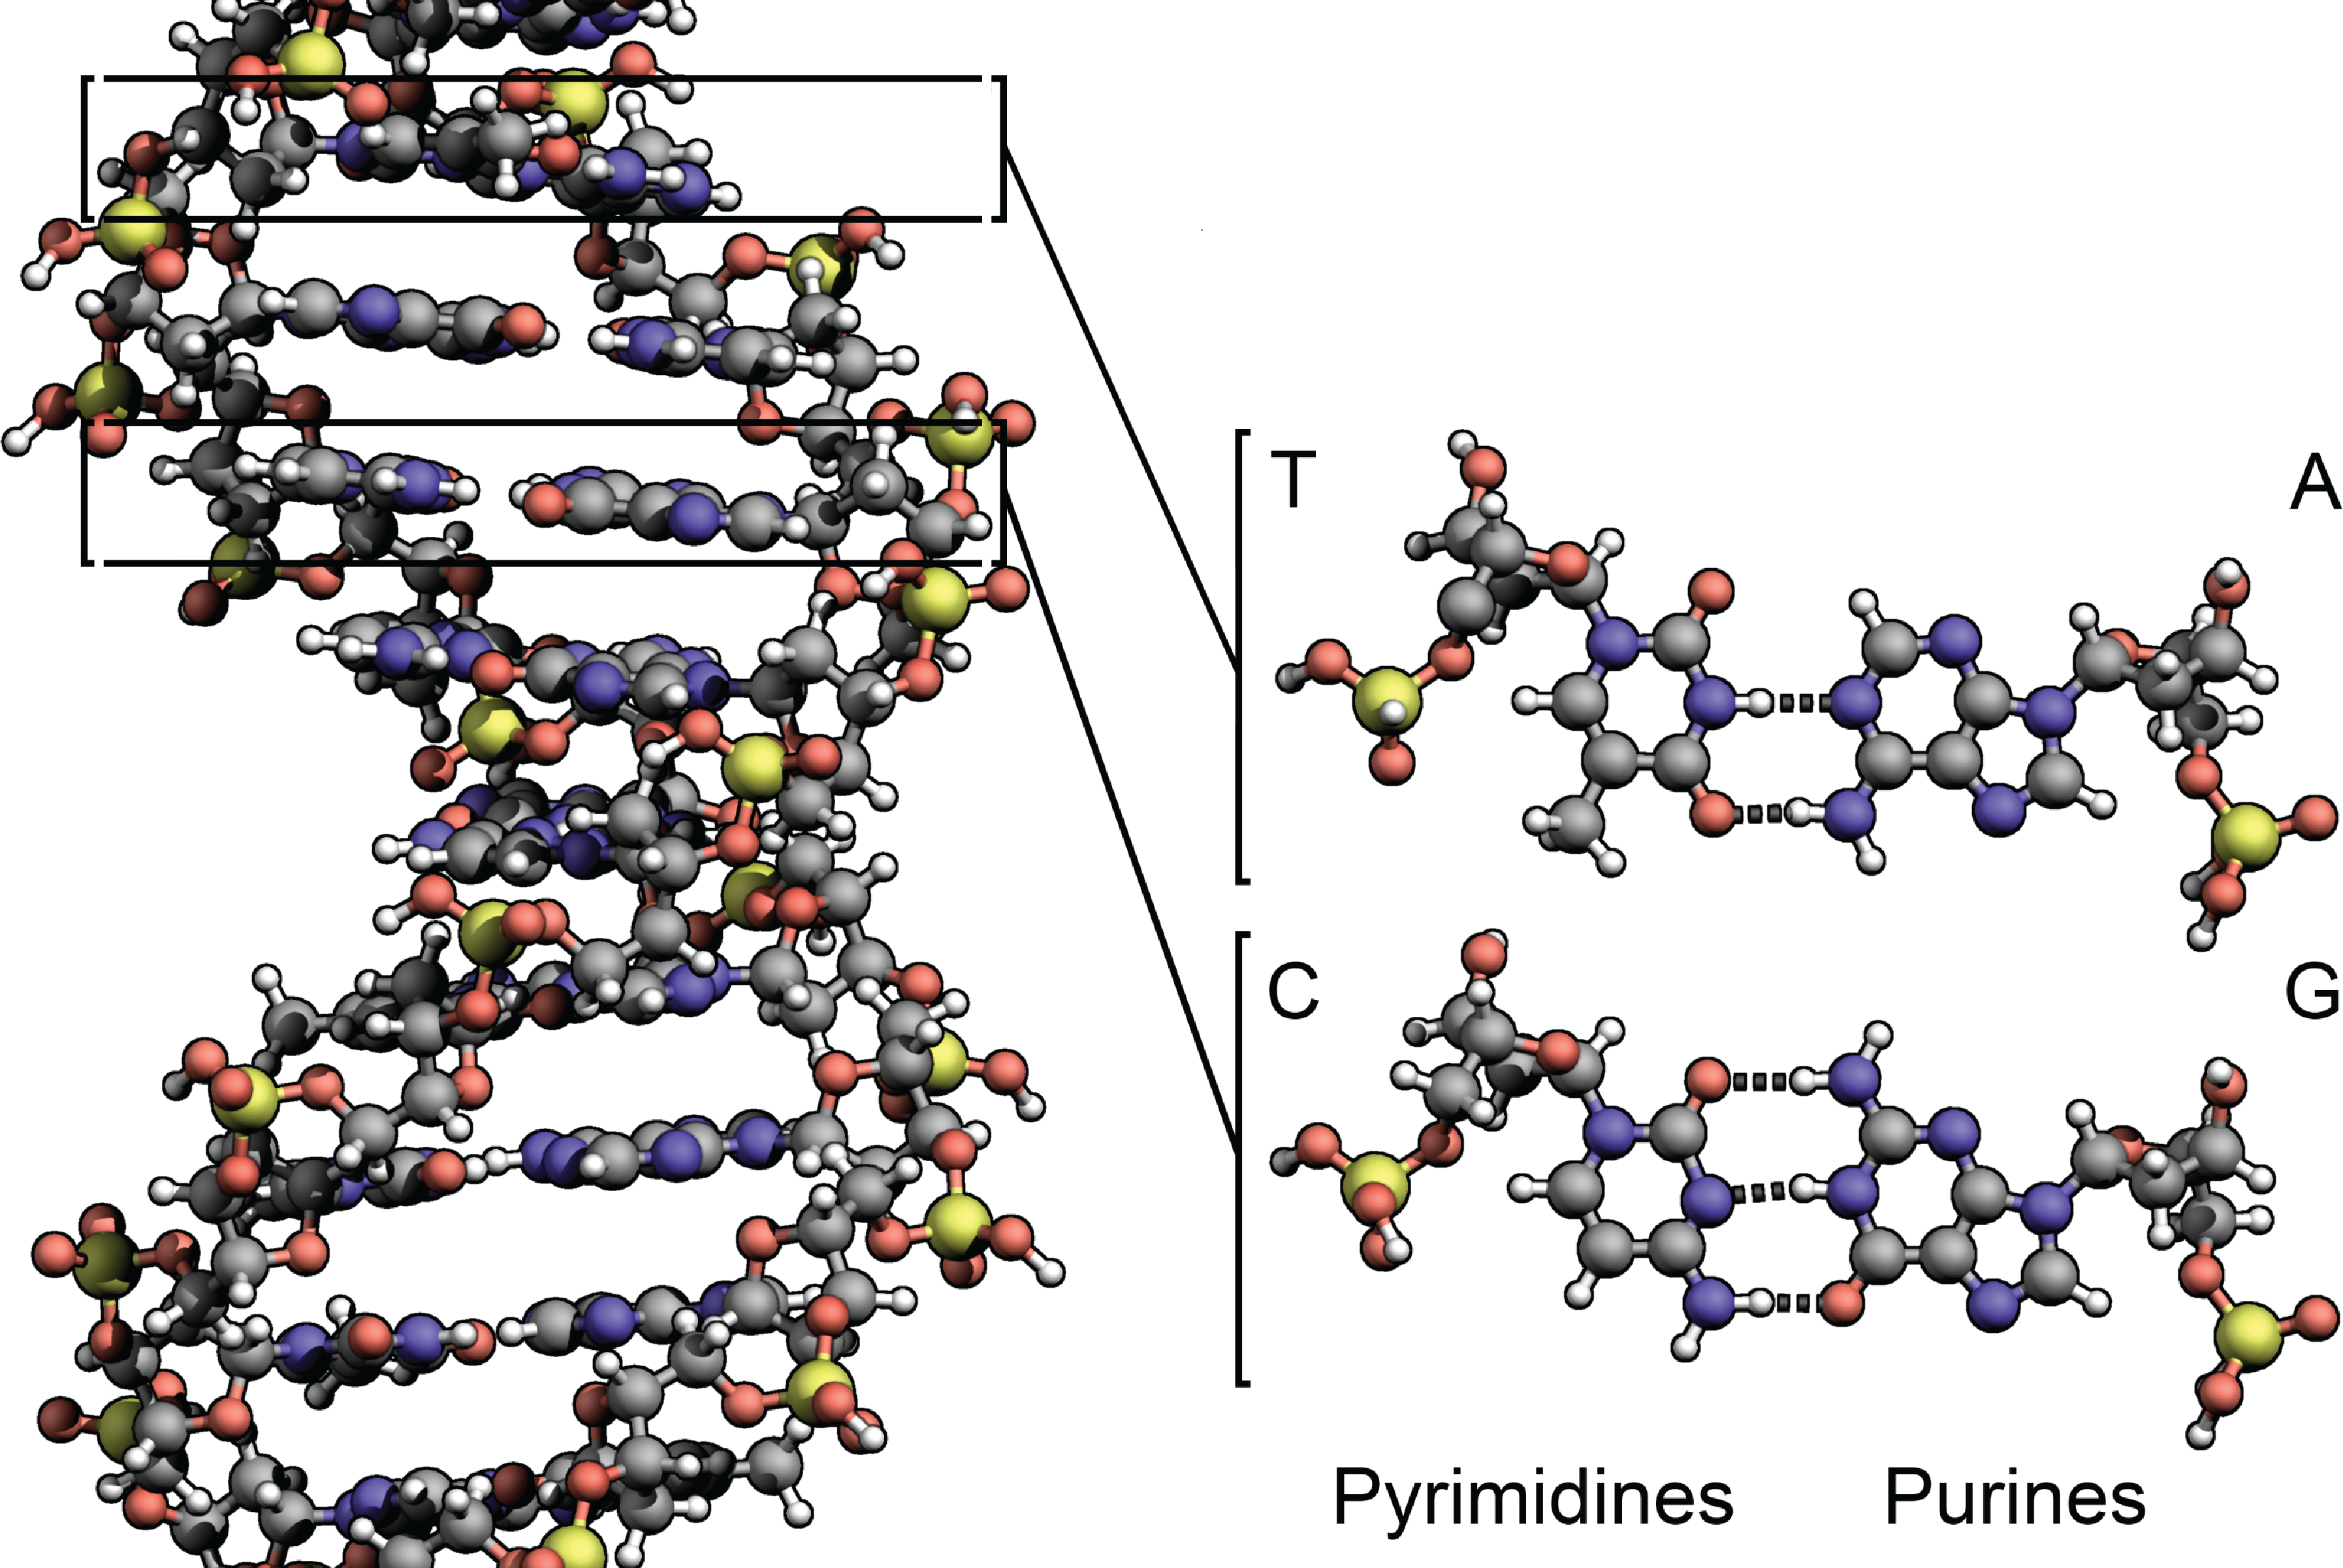
\includegraphics[width=0.4\textwidth]{fig03/dna_watson_crick_pair.png}
  \caption{Watson-Crick pairs (source: \href{https://commons.wikimedia.org/w/index.php?curid=15027555}{Zephyris, Wikimedia Commons})}
\end{figure}

%
% NEWPAGE
%
\newpage

\noindent \textbf{Example of score matrix for DNA pairs} \\
\noindent The matrix reflects the difference of hydrogen bonds.

\begin{figure}[H]
  \centering
      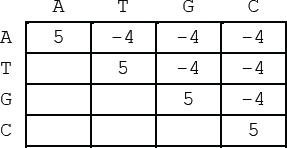
\includegraphics[width=0.3\textwidth]{fig03/example_dna_score_matrix.png}
\end{figure}

\noindent \textbf{Example of DP for DNA pairs} \\
\noindent You can use DP to find a DNA alignment with Watson-Crick pairs. For instance, the DP table below is used to solve the optimal alignment for two DNA sequences: q = AC and d = GT with gap penalty g = 4.

\begin{multicols}{2}
DP table:
\begin{figure}[H]
  \centering
      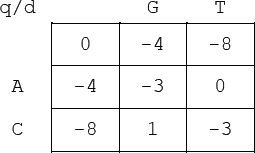
\includegraphics[width=0.25\textwidth]{fig03/example_watson_crick_alignment.png}
\end{figure}

Alignment:
\begin{verbatim}
    q: AC-
    d: -GT
\end{verbatim}

\end{multicols} 

%
% RNA pairs (Watson-Crick pairs)
%
\subsubsection*{RNA pairs}
A single stand of RNA can form a 3D structure that has a biological function. The secondary structure of RNA is a two-dimensional representation of the structure. 

\begin{figure}[H]
  \centering
      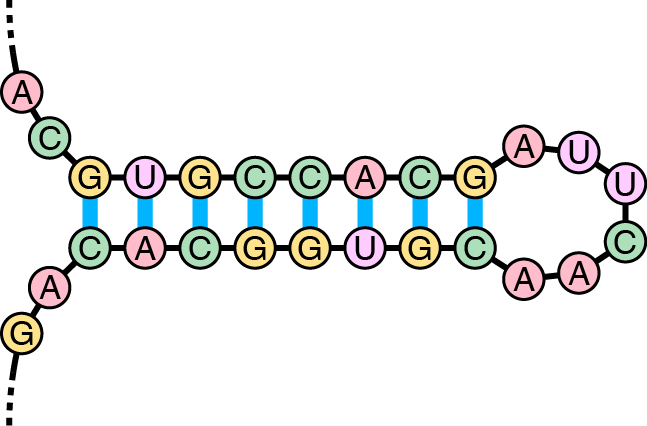
\includegraphics[width=0.3\textwidth]{fig03/rna_stem_loop.png}
  \caption{RNA stem-loop (source: \href{https://commons.wikimedia.org/w/index.php?curid=815268}{Sakurambo, Wikimedia Commons})}
\end{figure}

\noindent \textbf{Wobble pairs} \\
\noindent Wobble pairs are not canonical Watson-Crick pairs, but they can still form hydrogen bonds.

\begin{figure}[H]
  \centering
      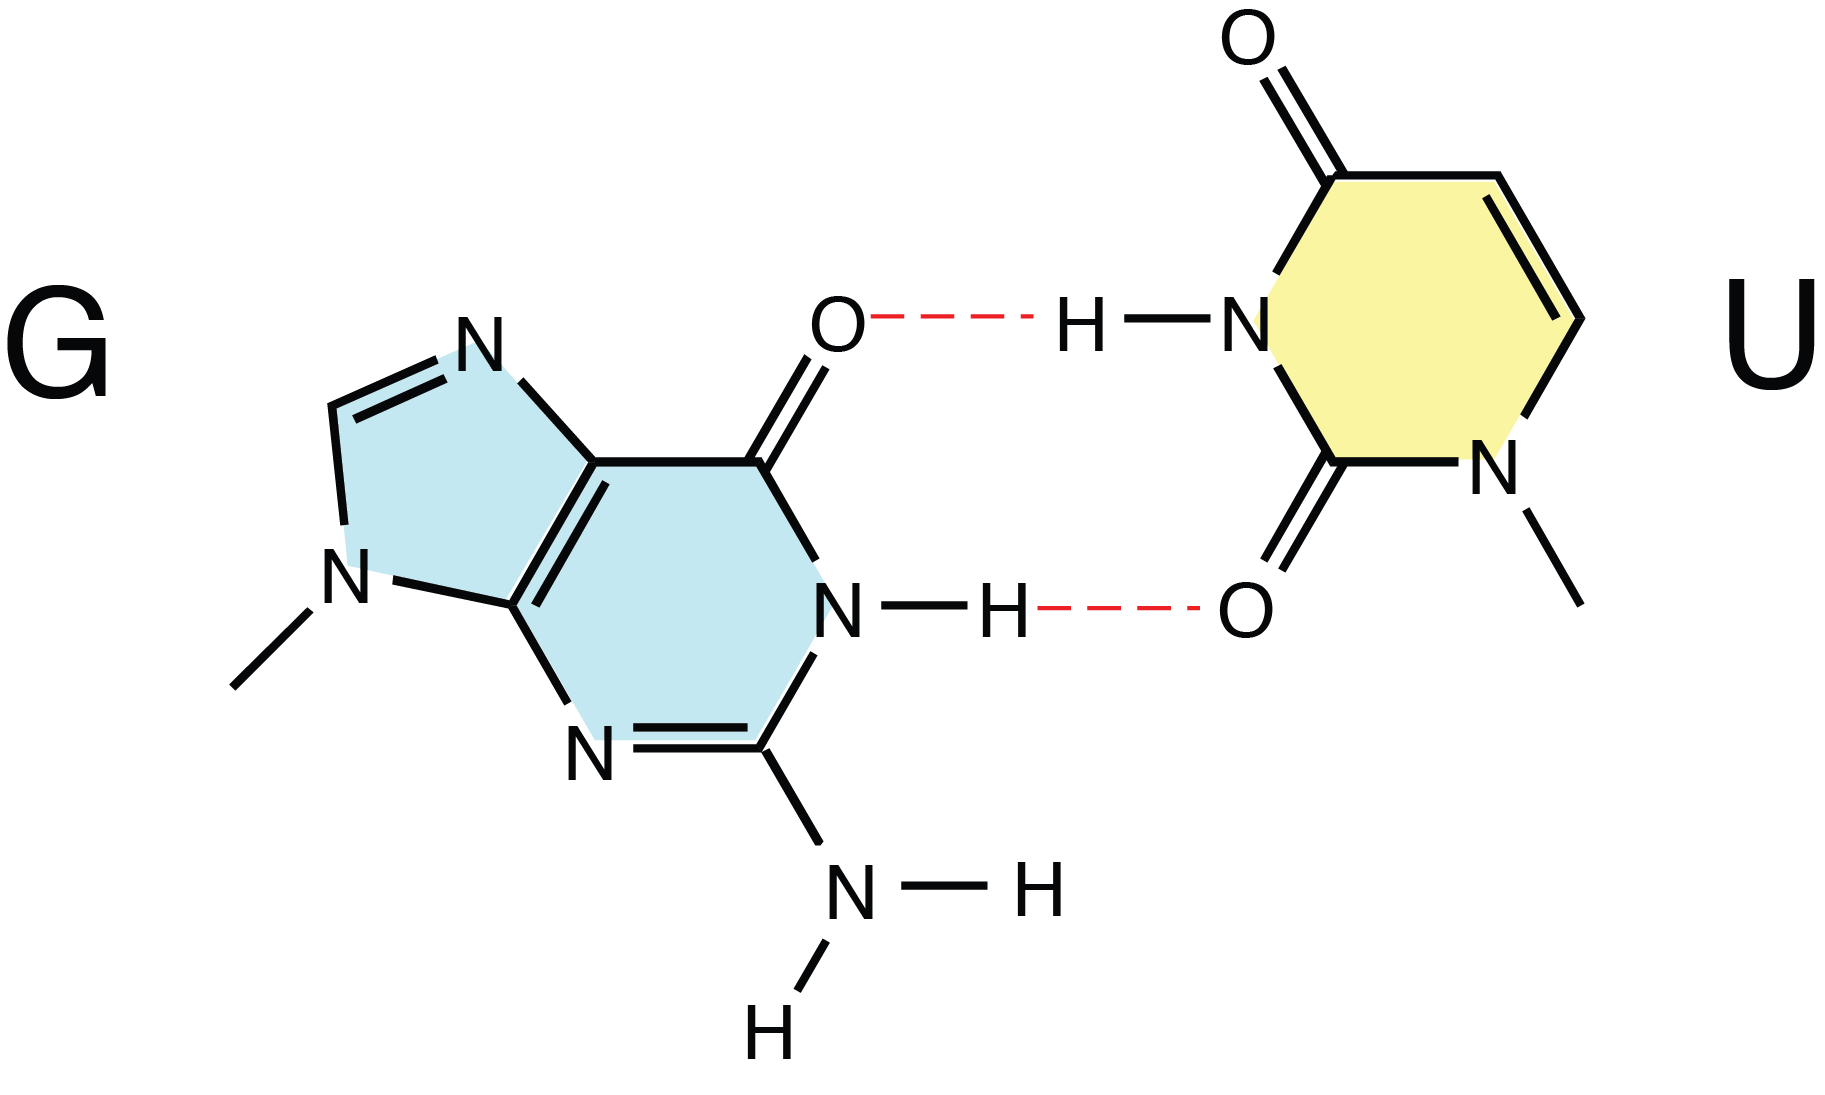
\includegraphics[width=0.3\textwidth]{fig03/rna_gu_wobble.png}
  \caption{GU wobble pairs \newline (modified  from the original version by \href{https://commons.wikimedia.org/w/index.php?curid=2636730}{Fdardel, Wikimedia Commons})}
\end{figure}

\noindent \textbf{Example of DP for RNA pairs} \\
\noindent You can form the following DP table for two RNA sequences: q = AU and d = UGA with gap penalty g = 9.
\begin{multicols}{2}
DP table:
\begin{figure}[H]
  \centering
      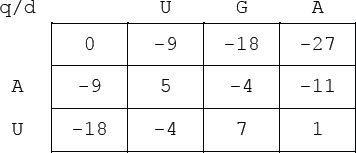
\includegraphics[width=0.25\textwidth]{fig03/example_rna_alignment.png}
\end{figure}

Alignment:
\begin{verbatim}
    q: A-U
    d: UGA
\end{verbatim}

\end{multicols} 

%
% Similarity of protein sequences
%
\subsubsection*{Similarity of protein sequences}
Amino acids can be categorized into several groups by their properties. Proteins alignments often need to take these properties into consideration.

\begin{figure}[H]
  \centering
      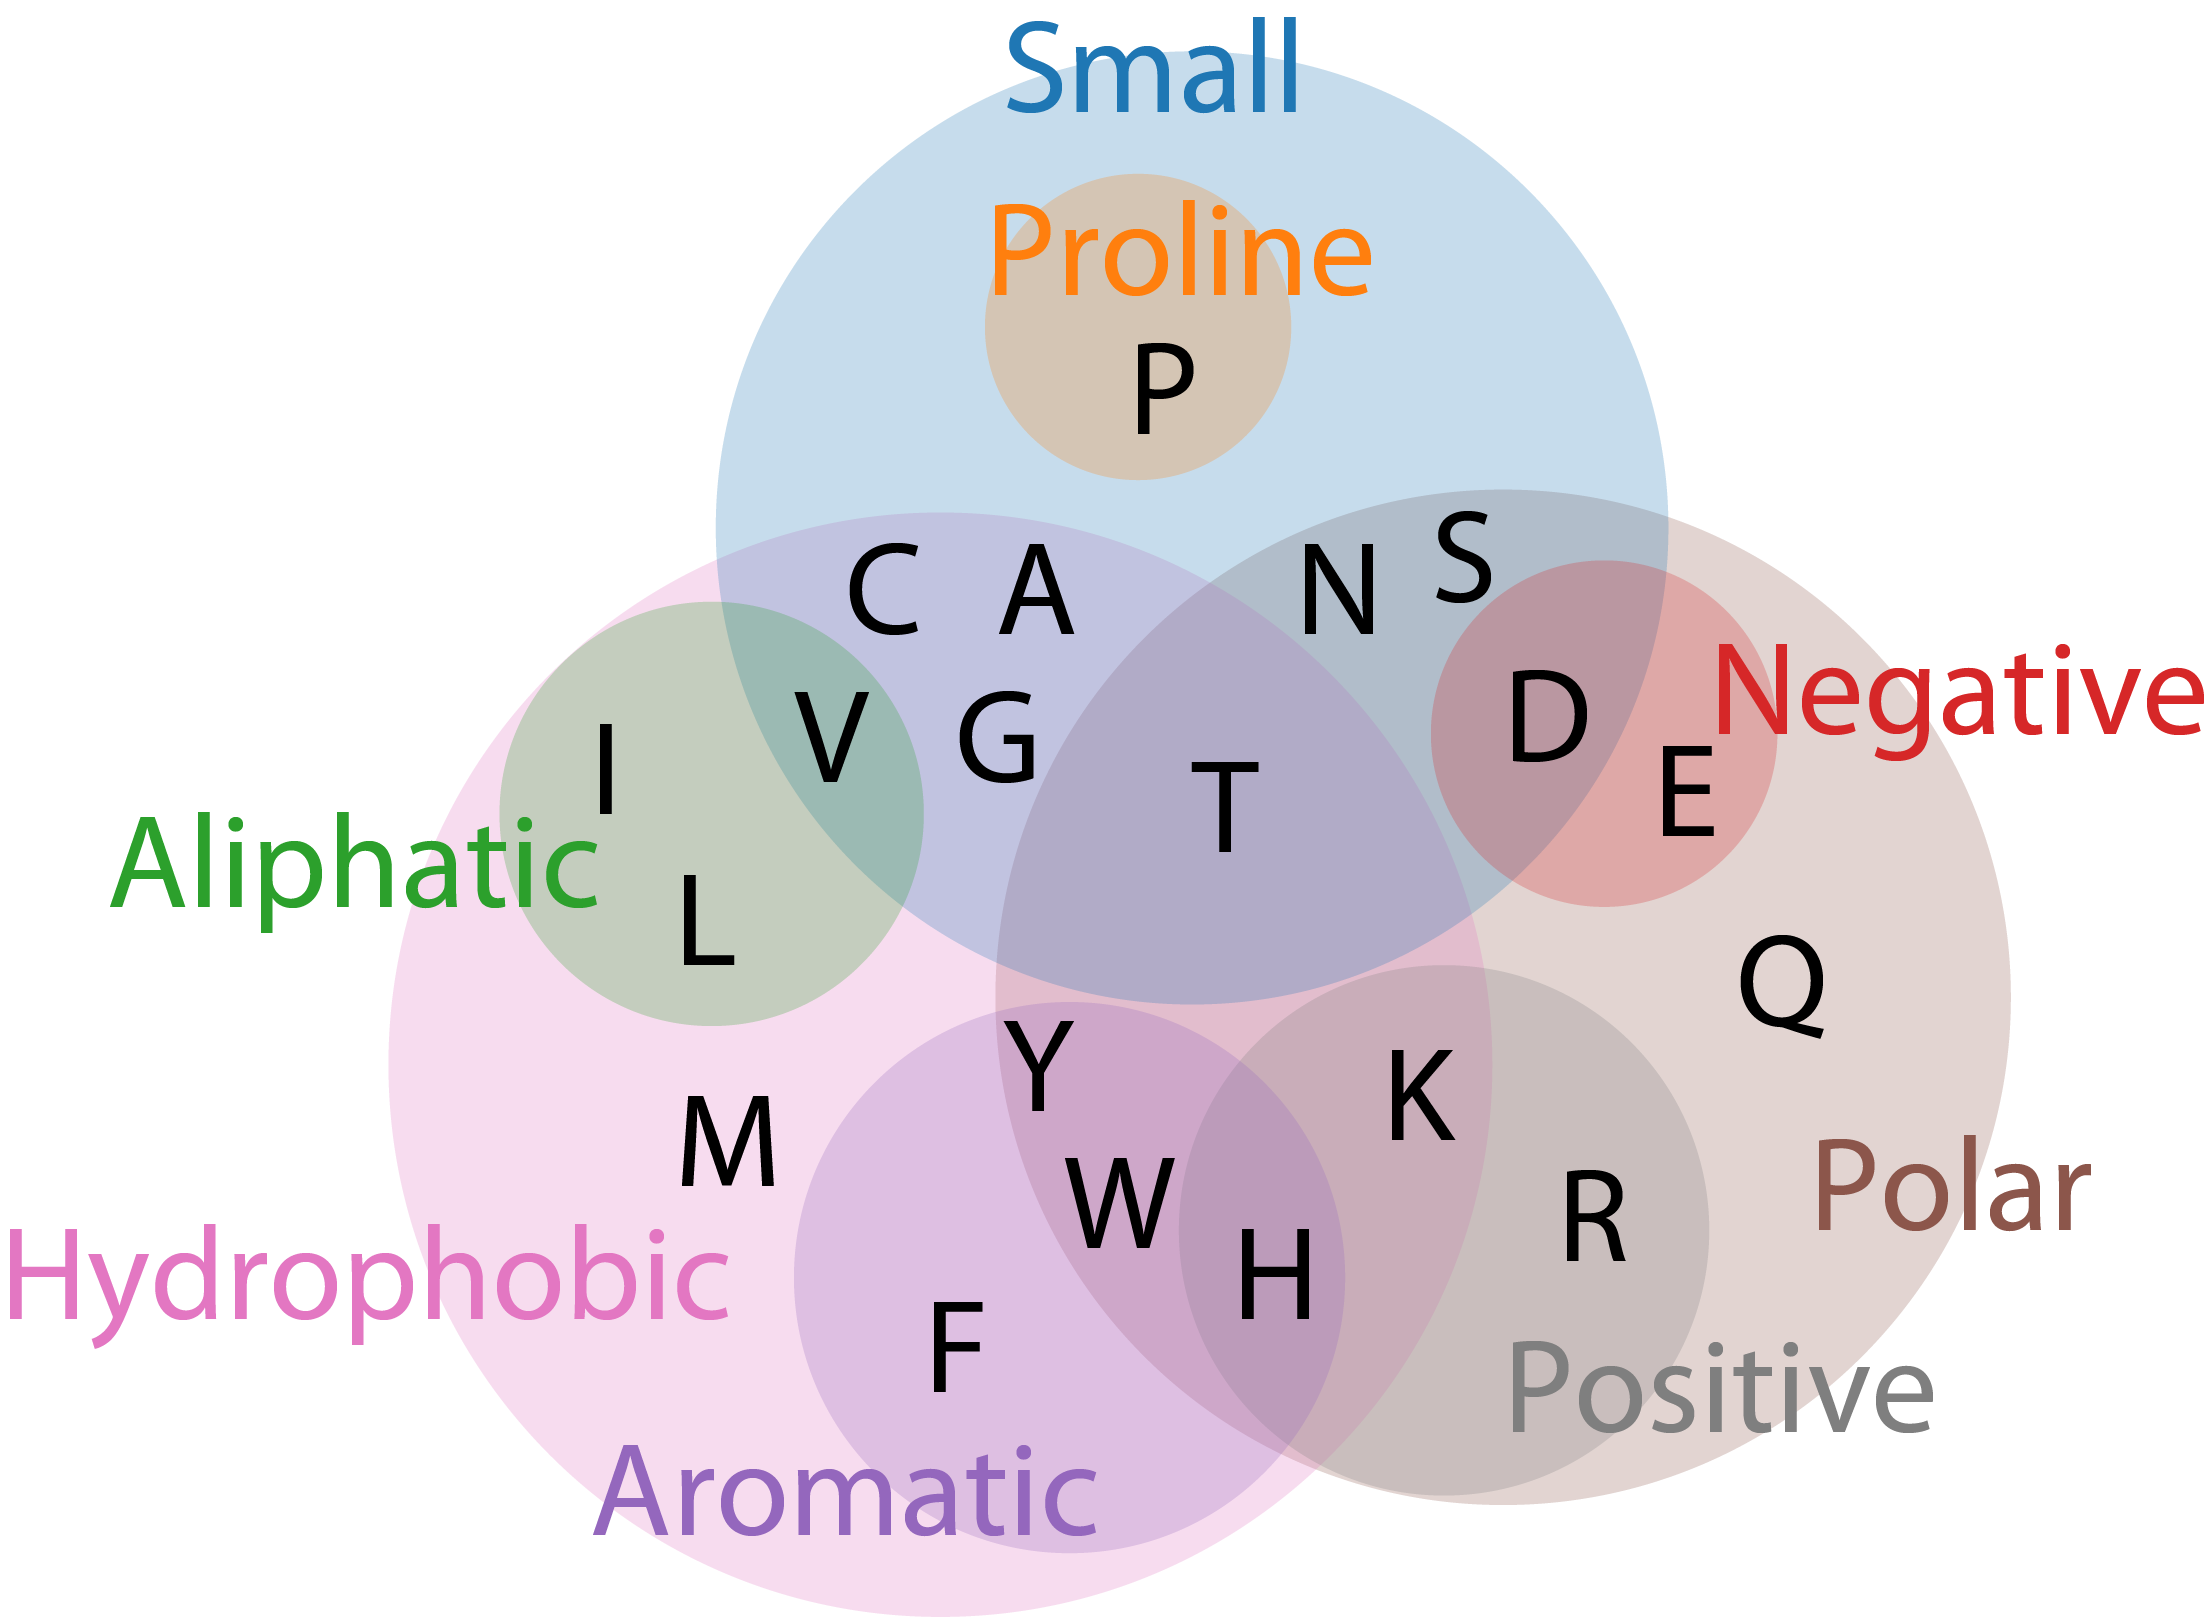
\includegraphics[width=0.3\textwidth]{fig03/amino_acid_properties.png}
  \caption{Venn diagram of amino acid properties }
\end{figure}

\noindent
\textbf{Example of a protein score matrix}\\
It can be used to compare the similarity between two protein sequences.

\begin{table}[!ht]
\footnotesize
\centering

\label{my-label}
\begin{tabular}{lllllllllllllllllllll}
   & \textbf{A }  & \textbf{R}   & \textbf{N}   & \textbf{D }  & \textbf{C}   & \textbf{Q}   & \textbf{E}   & \textbf{G}   & \textbf{H }  & \textbf{I}   & \textbf{L}   & \textbf{K}   & \textbf{M}   & \textbf{F}   & \textbf{P}   & \textbf{S}   & \textbf{T}   & \textbf{W}   & \textbf{Y}   & \textbf{V}   \\
\textbf{A} & 13  & 6   & 9   & 9   & 5   & 8   & 9   & 12  & 6   & 8   & 6   & 7   & 7   & 4   & 11  & 11  & 11  & 2   & 4   & 9   \\
\textbf{R} & 3   & 17  & 4   & 3   & 2   & 5   & 3   & 2   & 6   & 3   & 2   & 9   & 4   & 1   & 4   & 4   & 3   & 7   & 2   & 2   \\
\textbf{N} & 4   & 4   & 6   & 7   & 2   & 5   & 6   & 4   & 6   & 3   & 2   & 5   & 3   & 2   & 4   & 5   & 4   & 2   & 3   & 3   \\
\textbf{D} & 5   & 4   & 8   & 11  & 1   & 7   & 10  & 5   & 6   & 3   & 2   & 5   & 3   & 1   & 4   & 5   & 5   & 1   & 2   & 3   \\
\textbf{C} & 2   & 1   & 1   & 1   & 52  & 1   & 1   & 2   & 2   & 2   & 1   & 1   & 1   & 1   & 2   & 3   & 2   & 1   & 4   & 2   \\
\textbf{Q} & 3   & 5   & 5   & 6   & 1   & 10  & 7   & 3   & 7   & 2   & 3   & 5   & 3   & 1   & 4   & 3   & 3   & 1   & 2   & 3   \\
\textbf{E }& 5   & 4   & 7   & 11  & 1   & 9   & 12  & 5   & 6   & 3   & 2   & 5   & 3   & 1   & 4   & 5   & 5   & 1   & 2   & 3   \\
\textbf{G} & 12  & 5   & 10  & 10  & 4   & 7   & 9   & 27  & 5   & 5   & 4   & 6   & 5   & 3   & 8   & 11  & 9   & 2   & 3   & 7   \\
\textbf{H} & 2   & 5   & 5   & 4   & 2   & 7   & 4   & 2   & 15  & 2   & 2   & 3   & 2   & 2   & 3   & 3   & 2   & 2   & 3   & 2   \\
\textbf{I }& 3   & 2   & 2   & 2   & 2   & 2   & 2   & 2   & 2   & 10  & 6   & 2   & 6   & 5   & 2   & 3   & 4   & 1   & 3   & 9   \\
\textbf{L} & 6   & 4   & 4   & 3   & 2   & 6   & 4   & 3   & 5   & 15  & 34  & 4   & 20  & 13  & 5   & 4   & 6   & 6   & 7   & 13  \\
\textbf{K} & 6   & 18  & 10  & 8   & 2   & 10  & 8   & 5   & 8   & 5   & 4   & 24  & 9   & 2   & 6   & 8   & 8   & 4   & 3   & 5   \\
\textbf{M} & 1   & 1   & 1   & 1   & 0   & 1   & 1   & 1   & 1   & 2   & 3   & 2   & 6   & 2   & 1   & 1   & 1   & 1   & 1   & 2   \\
\textbf{F} & 2   & 1   & 2   & 1   & 1   & 1   & 1   & 1   & 3   & 5   & 6   & 1   & 4   & 32  & 1   & 2   & 2   & 4   & 20  & 3   \\
\textbf{P} & 7   & 5   & 5   & 4   & 3   & 5   & 4   & 5   & 5   & 3   & 3   & 4   & 3   & 2   & 20  & 6   & 5   & 1   & 2   & 4   \\
\textbf{S} & 9   & 6   & 8   & 7   & 7   & 6   & 7   & 9   & 6   & 5   & 4   & 7   & 5   & 3   & 9   & 10  & 9   & 4   & 4   & 6   \\
\textbf{T} & 8   & 5   & 6   & 6   & 4   & 5   & 5   & 6   & 4   & 6   & 4   & 6   & 5   & 3   & 6   & 8   & 11  & 2   & 3   & 6   \\
\textbf{W} & 0   & 2   & 0   & 0   & 0   & 0   & 0   & 0   & 1   & 0   & 1   & 0   & 0   & 1   & 0   & 1   & 0   & 55  & 1   & 0   \\
\textbf{Y} & 1   & 1   & 2   & 1   & 3   & 1   & 1   & 1   & 3   & 2   & 2   & 1   & 2   & 15  & 1   & 2   & 2   & 3   & 31  & 2   \\
\textbf{V} & 7   & 4   & 4   & 4   & 4   & 4   & 4   & 4   & 5   & 4   & 15  & 10  & 4   & 10  & 5   & 5   & 5   & 72  & 4   & 17 
\end{tabular}
\caption{Mutation probability matrix for the evolutionary distance of 250 PAMs (in percentage) (Chapter 22: A model of evolutionary change in proteins, Dayhoff and Schwartz, Atlas of Protein Sequence and Structure, 1978)}
\end{table}

%
% Exercise \thesection.1
%
\subsubsection*{Exercise \thesection.1}
\begin{enumerate}
\item Use the DNA score matrix below with g = 10 and find the optimal alignment for q = TG and d = TCG.

\begin{figure}[H]
  \centering
      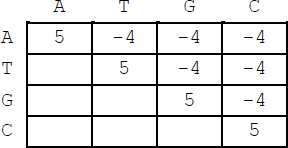
\includegraphics[width=0.25\textwidth]{fig03/dna_matrix_exercise.png}
\end{figure}

\item The 250 PAM mutation matrix above can not directly be used for global alignments. Explain what kind of matrix you need for calculating  alignment scores.
\end{enumerate}

\bigskip 

%\end{document}

%\documentclass[12pt]{article}
%\usepackage[a4paper, margin=1in]{geometry} 
%\usepackage{graphicx} 
%\usepackage{hyperref}
%\usepackage{float}
%\usepackage{multicol}
%\usepackage[font=small, labelfont=bf]{caption}
%
%\begin{document}

%
% Extension of gap penalties
%
\subsection{Extension of gap penalties}

%
% Types of gap penalties
%
\subsubsection*{Types of gap penalties}
Three types of gap penalties can be considered when creating an alignment. They treat a gap penalty differently depending on the gap length.

\begin{itemize}
\item Linear
\item Affine
\item Constant
\end{itemize}

%
% Gap penalty notation
%
\subsubsection*{Gap penalty notation}
\begin{itemize}
\item $g$: single gap penalty
\item $l$: length of a gap
\item $g_l$: gap penalty of length l
\item $g_{open}$: initial gap penalty
\item $g_{extend}$: extended gap penalty
\end{itemize}

%
% Linear gap penalty
%
\subsubsection*{Linear gap penalty}
It is the same as our simple scoring scheme. It treats a gap with multiple blanks as a result of several mutations. A gap of length $l$ can be calculated as: $g_l = g * l$.
\medskip 

\noindent
\textbf{Example of a gap of length 2}
\begin{verbatim}
    q: ACCCGT
    d: AC--GT
\end{verbatim}
The score of the gap (only the gap part) is 10 when $g$ = 5. 

%
% Affine gap penalty
%
\subsubsection*{Affine gap penalty}
It treats a gap with multiple blanks as a result of a single mutation. A gap with length $l$ can be calculated as: $g_l = g_{open} + (l – 1) * g_{extend}$.
\medskip 

\noindent
\textbf{Example of a gap of length 2}
\begin{verbatim}
    q: ACCCGT
    d: AC--GT
\end{verbatim}
The score of the gap (only the gap part) is 5.5 when $g_{open}$ and $g_{extend}$ are 5 and 0.5 respectively. 

%
% Constant gap penalty
%
\subsubsection*{Constant gap penalty}
It is similar to the affine gap penalty, but the score is independent form the gap length. A gap with length l can be calculated as: $g_l = g$ 
\medskip 

\noindent
\textbf{Example of a gap of length 2}
\begin{verbatim}
    q: ACCCGT
    d: AC--GT
\end{verbatim}
The score of the gap (only the gap part) for the alignment above is 5 when $g$ = 5. 

%
% Exercise \thesection.2
%
\subsubsection*{Exercise \thesection.2}
Calculate all three types of gap penalties for the gap in alignment 1 \& 2.

\begin{itemize}
\item $g$: 5
\item $g_{open}$: 5
\item $g_{extend}$: 0.5
\end{itemize}

\begin{multicols}{2}
\begin{verbatim}
Alignment 1
    q: CCCGG 
    d: CC-CG
\end{verbatim}

\begin{verbatim}
Alignment 2 
    q: CCCGG
    d: C---G
\end{verbatim}
\end{multicols}

%\end{document}

%\documentclass[12pt]{article}
%\usepackage[a4paper, margin=1in]{geometry} 
%\usepackage{graphicx} 
%\usepackage{hyperref}
%\usepackage{float}
%\usepackage{multicol}
%\usepackage{amsmath}
%\usepackage[font=small, labelfont=bf]{caption}
%
%\begin{document}

%
% Affine gap penalties with a single DP table
%
\subsection{Affine gap penalties with a single DP table}

%
% DP for general gap penalty
%
\subsubsection*{DP for general gap penalty}
We need to modify DP so that extra cells are checked to find the optimal score of a cell. 

%
% Cell update rule of general gap penalty
%
\subsubsection*{Cell update rule of general gap penalty}
\null \medskip  
\begin{equation*}
H_{i,j} =\max \left[H_{i-1,j-1} + R_{q_{i}d_{j}}, \quad \max_{1 \leq l \leq j}(H_{i,j-l} - g_l) ,  \quad \max_{1 \leq l \leq i}(H_{i-l,j} - g_l) \right]
\end{equation*}

%
% NEWPAGE
%
\newpage

\noindent
\textbf{Example of cell update}

\begin{multicols}{2}
Sequences:
\begin{verbatim}
    q: AG, d: ACG
\end{verbatim}
\vfill\null
\columnbreak

\noindent
Scoring scheme: \\
\null \quad $g_{open}$ = 1 \\
\null \quad $g_{extend}$ = 0.1 \\
\null \quad $R_{ab}$ = 1 for a = b \\ 
\null \quad $R_{ab}$ = 0 for a $\neq$ b \\ 

\end{multicols} 

\textbf{Update $H_{2,1}$}

\begin{figure}[H]
  \centering
      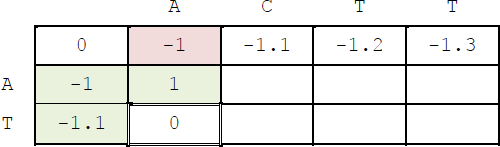
\includegraphics[width=0.5\textwidth]{fig03/dp_general_gap_example_1.png}
\end{figure}

\begin{itemize}
\item vertical:   $max(1 - 1, \quad -1 - 1 - 0.1) = 0$
\item horizontal: $-1.1 - 1 = -2.1$
\item diagonal: $-1 - 0 = -1$
\end{itemize}

\null \medskip 
\textbf{Update $H_{1,2}$}

\begin{figure}[H]
  \centering
      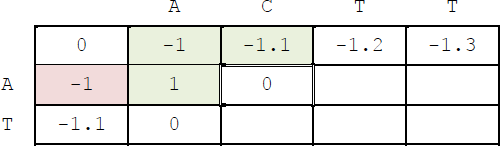
\includegraphics[width=0.5\textwidth]{fig03/dp_general_gap_example_2.png}
\end{figure}

\begin{itemize}
\item vertical: $-1.1 - 1 = -2.1$
\item horizontal: $max(1 - 1, \quad -1 - 1 - 0.1) = 0$
\item diagonal: $-1 - 0 = -1$
\end{itemize}

\null \medskip 
\textbf{Update $H_{1,3}$}

\begin{figure}[H]
  \centering
      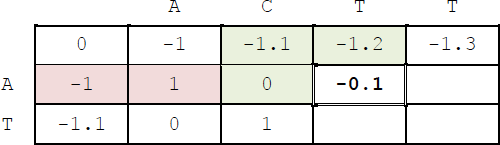
\includegraphics[width=0.5\textwidth]{fig03/dp_general_gap_example_3.png}
\end{figure}

\begin{itemize}
\item vertical: $-1.2 - 1 = -2.2$
\item horizontal: $max(0 - 1, \quad 1 - 1 - 0.1, \quad  -1 -1 - 0.1 - 0.1) = -0.1$
\item diagonal: $-1.1 - 0 = -1.1$
\end{itemize}


%
% Exercise \thesection.3
%
\subsubsection*{Exercise \thesection.3}
Complete the DP table below.

\begin{multicols}{2}
Sequences:
\begin{verbatim}
    q: AT, d: ACTT
\end{verbatim}
\vfill\null
\columnbreak

\noindent
Scoring scheme: \\
\null \quad $g_{open}$ = 1 \\
\null \quad $g_{extend}$ = 0.1 \\
\null \quad $R_{ab}$ = 1 for a = b \\ 
\null \quad $R_{ab}$ = 0 for a $\neq$ b \\ 

\end{multicols} 

\begin{figure}[H]
  \centering
      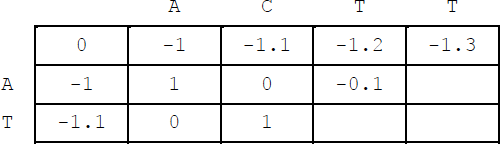
\includegraphics[width=0.5\textwidth]{fig03/dp_general_gap_exercise.png}
\end{figure}

%\end{document}

%\documentclass[12pt]{article}
%\usepackage[a4paper, margin=1in]{geometry} 
%\usepackage{graphicx} 
%\usepackage{hyperref}
%\usepackage{float}
%\usepackage{multicol}
%\usepackage{amsmath}
%\usepackage[font=small, labelfont=bf]{caption}
%
%\begin{document}

%
% Affine gap penalties with three DP tables
%
\subsection{Affine gap penalties with three DP tables}
DP can effectively solve affine gap penalties with three tables.

\begin{figure}[H]
  \centering
      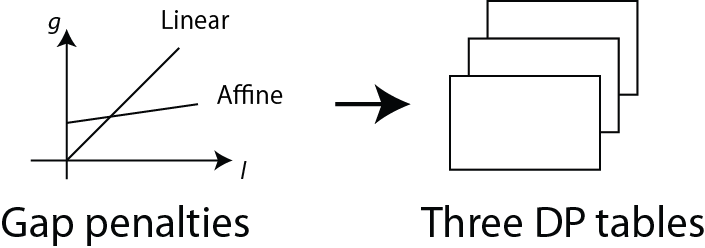
\includegraphics[width=0.4\textwidth]{fig03/three_dp_tables_for_affine.png}
  \caption{Affine gap penalties and three tables}
\end{figure}

%
% Three DP tables
%
\subsubsection*{Three DP tables}
We need to modify DP so that extra cells are checked to find the optimal score of a cell. 

\begin{itemize}
\item $E_{i,j}$: alignment ending with a gap extend (vertical)
\item $F_{i,j}$: alignment ending with a gap extend (horizontal)
\item $G_{i,j}$: alignment ending with a match/mismatch (diagonal)
\end{itemize}

%
% Cell update rule of the three tables
%
\subsubsection*{Cell update rule of the three tables}

\begin{align*}
E_{i,j} &= max(E_{i-1,j} - g_{extend}, \quad F_{i-1,j} - g_{open}, \quad G_{i-1,j} - g_{open}) \\
F_{i,j} &= max(E_{i,j-1} - g_{open}, \quad F_{i,j-1} - g_{extend}, \quad G_{i,j-1} - g_{open}) \\
G_{i,j} &= max(E_{i-1,j-1} + R_{q_{i}d_{j}}, \quad F_{i-1,j-1}+ R_{q_{i}d_{j}}, \quad G_{i-1,j-1} + R_{q_{i}d_{j}})
\end{align*}

\noindent You can calculate H only in the last cell.
\begin{align*}
H_{m,n} = max(E_{m,n}, F_{m,n}, G_{m,n})
\end{align*}

\begin{figure}[H]
  \centering
      \includegraphics[width=0.25\textwidth]{fig03/three_dp_tables_update_for_affine.png}
  \caption{Update a cell with E, F, and G}
\end{figure}

%
% NEWPAGE
%
%\newpage

%
% Recurrence rules when i = 0 and j = 0
%
\subsubsection*{Recurrence rules when i = 0 and j = 0}
\begin{figure}[H]
  \centering
      \includegraphics[width=0.75\textwidth]{fig03/affine_dp_special_cases.png}
\end{figure}
\null \medskip 

%
% Example of updating DP tables with affine gaps
%
\subsubsection*{Example of updating DP tables with affine gaps}
\begin{multicols}{2}
Sequences:
\begin{verbatim}
    q: AT, d: ACTT
\end{verbatim}
\vfill\null
\columnbreak

\noindent
Scoring scheme: \\
\null \quad $g_{open}$ = 1 \\
\null \quad $g_{extend}$ = 0.1 \\
\null \quad $R_{ab}$ = 1 for a = b \\ 
\null \quad $R_{ab}$ = 0 for a $\neq$ b \\ 

\end{multicols} 
 
\textbf{Initialization}
\begin{figure}[H]
  \centering
      \includegraphics[width=0.75\textwidth]{fig03/affine_dp_init.png}
\end{figure}
\null \medskip 

\textbf{Update the first row}
\begin{figure}[H]
  \centering
      \includegraphics[width=0.75\textwidth]{fig03/affine_dp_first_row.png}
\end{figure}
\null \medskip 

\textbf{Update the second row}
\begin{figure}[H]
  \centering
      \includegraphics[width=0.75\textwidth]{fig03/affine_dp_update_h.png}
\end{figure}
\null \medskip 

\textbf{Update H}
\begin{figure}[H]
  \centering
      \includegraphics[width=0.75\textwidth]{fig03/affine_dp_backtrack.png}
\end{figure}
\null \medskip 

\textbf{Backtrack}
\begin{figure}[H]
  \centering
      \includegraphics[width=0.75\textwidth]{fig03/affine_dp_backtrack.png}
\end{figure}
\null \medskip 

\textbf{Optimal alignment}
\begin{verbatim}
    q: A--T    Score: 0.9
    d: ACTT
\end{verbatim}

%
% Constant gap penalty
%
\subsubsection*{Constant gap penalty}
DP with constant gap penalty can be solved in the same way as the affine gap penalty.
\begin{figure}[H]
  \centering
      \includegraphics[width=0.25\textwidth]{fig03/gap_penalty_constant.png}
  \caption{Constant gap penalty}
\end{figure}

%\end{document}


%\documentclass[12pt]{article}
%\usepackage[a4paper, margin=1in]{geometry} 
%\usepackage{graphicx} 
%\usepackage{hyperref}
%\usepackage{float}
%\usepackage{multicol}
%\usepackage{amsmath}
%\usepackage[font=small, labelfont=bf]{caption}
%
%\begin{document}

%
% Sequence distance
%
\subsection{Sequence distance}
Distances can be also used to indicate the similarity of an alignment.

%
% Edit distance
%
\subsubsection*{Edit distance}
The Levenshtein distance is one of the most commonly used edit distances in computer science.
\begin{align*}
\mathrm{Insertion}: & \quad AC  \rightarrow AGC  & (\varepsilon  \rightarrow G) \\
\mathrm{Deletion}: & \quad ATC \rightarrow AC & (T \rightarrow \varepsilon) \\
\mathrm{Substitution}: & \quad AAA \rightarrow ATA &  (A \rightarrow T) 
\end{align*}

%
% Scoring scheme for Levenshtein distance
%
\subsubsection*{Scoring scheme for Levenshtein distance}
\begin{itemize}
\item $R_{ab}$ = 0 for a = b
\item $R_{ab}$ = -1 for a $\neq$ b
\item g = 1
\end{itemize}

%
% Distance from DP score
%
\subsubsection*{Distance from DP score}
Given the best score $T$ from DP, the edit distance $d$ is $-T$.
\bigskip  

\noindent
\textbf{Example of edit distance with DP}
\begin{multicols}{2}
\begin{figure}[H]
  \centering
      \includegraphics[width=0.4\textwidth]{fig03/dp_for_edit_distance.png}
\end{figure}
\vfill\null
\columnbreak

\vfill\null
\noindent $T = -1$ \\\\
\noindent $d = 1$

\end{multicols} 

%
% Metric space
%
\subsubsection*{Metric space}
The edit distance constitutes a metric space.
\begin{itemize}
\item $d_{xy} = 0$ for $x = y$ 
\item $d_{xy} > 0$ for $x \neq y$
\item $d_{xy} = d_{yx}$
\item $d_{xy} \leq d_{xz} + d_{zy}$ for any $z$ (the triangle inequality)
\end{itemize}

%
% Mutation and distance
%
\subsubsection*{Mutation and distance}
Mutations may occur several times on the same position.

\medskip 
\noindent
\textbf{Example of single mutations} \\

\noindent
$ACGT \rightarrow AGT \rightarrow ACT \rightarrow AGT \rightarrow AGCT$

\medskip 
\noindent
Four mutations have occurred, but the edit distance is 2.

%
% Mutation and distance
%
\subsubsection*{Distance per column}
It indicates the number of mutations per column (nucleotide/amino acid).

\bigskip 
$D = d / $(length of the longest sequence)

%
% Correction of distance
%
\subsubsection*{Correction of distance}
The distance can be adjusted. Below is a simple correction approach for protein sequences.

\bigskip 
$K=-\ln⁡(1-D-1/5 D^2 )$
\begin{figure}[H]
  \centering
      \includegraphics[width=0.3\textwidth]{fig03/adjust_distance.png}
      \caption{Correction of distance $D$}
\end{figure}

\medskip 
\noindent
\textbf{Example of distance correction} \\

$D = 0.5$

$K = -\ln⁡(1 - 0.5 - 1/5  \times 0.25 ) = -\ln(0.45) \approx 0.8⁡$

%\end{document}



\newpage

%
% Local alignment
%
\setcounter{figure}{0}
\setcounter{table}{0}
\section{Local alignment}
%\documentclass[12pt]{article}
%\usepackage[a4paper, margin=1in]{geometry} 
%\usepackage{graphicx} 
%\usepackage{hyperref}
%\usepackage{float}
%\usepackage{multicol}
%\usepackage[font=small, labelfont=bf]{caption}
%
%\begin{document}

%
% Local alignments
%
\subsection{Local alignments}
Local pairwise alignments are aligned pairs of sub--sequences that have centain level of similarities.

%
% Deiffrence between global and local alignments
%
\subsubsection*{Deiffrence between global and local alignments} 

\begin{figure}[H]
  \centering
      \includegraphics[width=0.75\textwidth]{fig04/global_and_local_alignments.png}
  \caption{Global and local alignments}
\end{figure}

%
% Elements of local alignment
%
\subsubsection*{Elements of local alignment}
\begin{itemize}
\item Segment: a substring of a sequence
\item Segment pair: a pair of segments
\item Local alignment: an alignment of a segment pair
\end{itemize}

%
% Alignment methods
%
\subsubsection*{Elements of local alignment}
\begin{itemize}
\item Dynamic programming (Smith--Waterman)
\item Dot matrix
\end{itemize}

%
% Applications
%
\subsubsection*{Applications}
\begin{itemize}
\item Sequence motifs
\item Conserved regions
\item Inverted repeats
\end{itemize}

\bigskip 

%\end{document}

%\documentclass[12pt]{article}
%\usepackage[a4paper, margin=1in]{geometry} 
%\usepackage{graphicx} 
%\usepackage{hyperref}
%\usepackage{float}
%\usepackage{multicol}
%\usepackage{amsmath}
%\usepackage[ruled]{algorithm2e}
%\usepackage{amssymb}
%\usepackage[font=small, labelfont=bf]{caption}
%
%\begin{document}

%
% Local alignment with DP
%
\subsection{Local alignment with DP}
Dynamic programming can be used to find local alignments.

%
% Requirements
%
\subsubsection*{Requirements}
\begin{itemize}
\item Find all local alignments between two sequences
\item Assign scores to all local alignments
\end{itemize}

%
% Modification of DP for local alignments
%
\subsubsection*{Modification of DP for local alignments}
\begin{itemize}
\item The minimum alignment score must be 0
\item Some entries of the score matrix should be negative
\item Backtracking also needs to be modified
\end{itemize}

%
% Update rule of DP cells
%
\subsubsection*{Update rule of DP cells}
\begin{align*}
H_{i,j}^{(0)} &= H_{i-1,j} - g &(vertical) \\
H_{i,j}^{(1)} &= H_{i,j-1} - g	&(horizontal) \\
H_{i,j}^{(2)} &= H_{i-1,j-1} + R_{a,b} &(diagonal) \\
H_{i,j}^{(2)} &= 0 &(minimum \, score)
\end{align*}

%
% Example of cell update
%
\subsubsection*{Example of cell update}
\begin{multicols}{2}
\begin{figure}[H]
  \centering
      \includegraphics[width=0.3\textwidth]{fig04/local_alignment_cell_update.png}
\end{figure}

\noindent Scoring scheme: \\ 
\null \quad Match: 0.5 \\ 
\null \quad Mismatch: -0.3 \\ 
\null \quad Gap penalty: 0.5

\end{multicols} 

\begin{align*}
H_{i,j}^{(0)} &=  -0.1 &\hfill &(vertical) \\
H_{i,j}^{(1)} &= -0.3 &\hfill &(horizontal) \\
H_{i,j}^{(2)} &= -0.2 &\hfill &(diagonal) \\
H_{i,j}^{(2)} &= 0 & \checkmark &(minimum \, score)
\end{align*}
\medskip 

%
% Backtracking 
%
\subsubsection*{Backtracking for local alignments}
It starts from the cells with the maximum score instead of the right bottom cell.

\begin{itemize}
\item Start cells: cells with the maximum score 
\item End cells: cells with 0
\end{itemize}

\noindent
\textbf{N.B.} the end cell with score 0 should not be included in the alignment.

%
% Example of backtracking
%
\subsubsection*{Example of backtracking}

\begin{figure}[H]
  \centering
      \includegraphics[width=0.7 \textwidth]{fig04/local_alignment_backtrack.png}
\end{figure}

\medskip 

%
% Pseudo-code of local alignment with DP
%
\subsubsection*{Pseudo-code of updating DP table for local alignment}
The cells in the first row and the first column are initialized with 0.

\begin{algorithm}[H]
  \SetKwInOut{HAB}{$\mathrm{H_{i,j}}$}
  \SetKwInOut{RAB}{$\mathrm{R_{a,b}}$}
  \SetKwInOut{G}{$\mathrm{g}$}
  \SetKwData{dRAB}{$\mathrm{R_{a,b}}$}
  \SetKwData{dG}{$\mathrm{g}$}
  
  \BlankLine
    
  \HAB{Dynamic programming table}
  \RAB{Match/mismatch scores}
  \G{Gap penalty}
  
  \BlankLine \BlankLine
  
  \tcp{Initialization}
  \For{$i \leftarrow 0$ \KwTo $m$}{
    $\mathrm{H_{i,0}}$ $\leftarrow$ $\mathbf{0} $\;
  }
  \For{$j \leftarrow 1$ \KwTo $n$}{
    $\mathrm{H_{0,j}}$ $\leftarrow$ $\mathbf{0} $\;
  }
  
  \BlankLine \BlankLine
    
  \tcp{Main loop for table update}
  \For{$i \leftarrow 1$ \KwTo $m$}{
    \For{$j \leftarrow 1$ \KwTo $n$}{
      $\mathrm{H_{i,j}}$ $\leftarrow$ $max(\mathrm{\mathbf{0}, H_{i-1,j}} - \dG, \mathrm{H_{i,j-1}} - \dG, \mathrm{H_{i-1,j-1}}$ + \dRAB)\;
    }
  }
  
  \SetAlgoRefName{\thesection.1}
  \caption{Update dynamic programming table for global alignment}

\end{algorithm}

%
% Exercise \thesection.1
%
\subsubsection*{Exercise \thesection.1}
	
Use DP to find a local alignment.

\begin{multicols}{2}
\begin{figure}[H]
  \centering
      \includegraphics[width=0.4\textwidth]{fig04/local_alignment_exercise.png}
\end{figure}

\noindent Scoring scheme: \\ 
\null \quad Match: 0.2 \\ 
\null \quad Mismatch: -0.2 \\ 
\null \quad Gap penalty: 0.2

\end{multicols} 

\bigskip 

%\end{document}

%\documentclass[12pt]{article}
%\usepackage[a4paper, margin=1in]{geometry} 
%\usepackage{graphicx} 
%\usepackage{hyperref}
%\usepackage{float}
%\usepackage{multicol}
%\usepackage{amsmath}
%\usepackage[ruled]{algorithm2e}
%\usepackage{amssymb}
%\usepackage[font=small, labelfont=bf]{caption}
%
%\begin{document}

%
% Dot matrix
%
\subsection{Dot matrix}
Using a dot matrix is an effective and easy way to find local similarities.

%
% Basic concept
%
\subsubsection*{Basic concept}
It uses an $m \times n$ binary matrix from two sequences.

\begin{itemize}
\item A dot: match
\item Empty: mismatch
\end{itemize}

%
% Example of dot matrix
%
\subsubsection*{Example of dot matrix}
\begin{verbatim}
    q: ACATTAG, d: CATTTAGG
\end{verbatim}

\begin{figure}[H]
  \centering
      \includegraphics[width=0.3\textwidth]{fig04/dot_matrix.png}
  \caption{Dot matrix of $7 \times 8$}
\end{figure}

\noindent
It is easy to find segment pairs with a dot matrix. Contiguous dots along diagonals indicate local alignments. It is also easy to find other similarities. For instance, contiguous dots along anti-diagonals indicate reversed substrings.

%
% Filtering of dot matrix
%
\subsubsection*{Filtering of dot matrix}
Dot matrices usually get noisy with too many dots.  Overlapping windows are usually applied to reduce the noise.

\bigskip 
\noindent
\textbf{Example of filtering}

\begin{figure}[H]
  \centering
      \includegraphics[width=0.3\textwidth]{fig04/dot_matrix_filtered.png}
  \caption{Filtered dot matrix with window size 3 and threshold 3.}
\end{figure}

%
% Exercise \thesection.2
%
\subsubsection*{Exercise \thesection.2}
Find local similarities between two DNA sequences, \verb|q: GATTACA| and \verb|d: GGATTTAC|.

\begin{enumerate}
\item Create a dot matrix for the two sequences.
\item Filter dots with overlapping windows size 3 and threshold 3.
\end{enumerate}

\bigskip 

%\end{document}


\newpage

%
% Database search
%
\setcounter{figure}{0}
\setcounter{table}{0}
\section{Database search}
%\documentclass[12pt]{article}
%\usepackage[a4paper, margin=1in]{geometry} 
%\usepackage{graphicx} 
%\usepackage{hyperref}
%\usepackage{float}
%\usepackage{multicol}
%\usepackage{multirow}
%\usepackage[font=small, labelfont=bf]{caption}
%
%\begin{document}

%
% Biological databases
%
 \subsection{Biological databases}
Biological databases contain biological information, mainly collected from molecular biology experiments, life science literature, and bioinformatics analyses.

%
% Categories of databases
%
\subsubsection*{Categories of databases} 
Annual \href{http://nar.oxfordjournals.org}{Nucleic Acids Research} database issue includes the following database categories.

\begin{itemize}
\item Nucleotide Sequence Databases
\item RNA sequence databases
\item Protein sequence databases
\item Structure Databases
\item Proteomics Resources
\item Human and other Vertebrate Genomes
\item Genomics Databases (non-vertebrate)
\item Plant databases
\item Human Genes and Diseases
\item Metabolic and Signaling Pathways
\item Immunological databases
\item ...
\end{itemize}

%
% GenBank
%
\subsubsection*{GenBank} 
\begin{itemize}
\item A comprehensive database of publicly available nucleotide sequences
\item Produced and maintained by NCBI (National Center for Biotechnology Information, URL: \href{http://www.ncbi.nlm.nih.gov}{http://www.ncbi.nlm.nih.gov})
\end{itemize}

\begin{figure}[H]
  \centering
      \includegraphics[width=0.6 \textwidth]{fig05/genebank_stat.png}
  \caption{Growth of GenBank and WGS (source: \href{http://www.ncbi.nlm.nih.gov/genbank/statistics}{NCBI})}
\end{figure}

%
% UniProt
%
\subsubsection*{UniProt} 
\begin{itemize}
\item A central repository of protein data from Swiss-Prot, TrEMBL, and PIR-PSD databases
\item Maintained by the UniProt consortium
\end{itemize}

%
% Sequence data 
%
\subsubsection*{Sequence data} 
\begin{itemize}
\item Identifier
\item Sequence
\end{itemize}

\noindent
\textbf{Data format of sequence data} \\
FASTA is the most popular format for sequence data.
\begin{figure}[H]
  \centering
      \includegraphics[width=\textwidth]{fig05/fasta.png}
\end{figure}

%
% Annotation data
%
\subsubsection*{Annotation data} 
Sequences databases usually contain annotations in addition to sequences. 

\begin{itemize}
\item Notes and descriptions of important regions and components
\item Meta data
\end{itemize}

\noindent
\textbf{Data format of annotation data} \\
Annotation data can be downloaded in many different formats. GFF is one of the popular file formats for storing genomic features.
\begin{figure}[H]
  \centering
      \includegraphics[width=\textwidth]{fig05/gff3.png}
\end{figure}

%
% Tools
%
\subsubsection*{Tools}
Many database tools are available for various purposes.
 
\noindent
\textbf{Search tools for sequence databases}
\begin{itemize}
\item BLAST at NCBI (\href{http://blast.ncbi.nlm.nih.gov/Blast.cgi}{http://blast.ncbi.nlm.nih.gov/Blast.cgi})
\item BLAT/BLAST at Ensembl (\href{http://www.ensembl.org/Multi/Tools/Blast}{http://www.ensembl.org/Multi/Tools/Blast})
\end{itemize}

\noindent
\textbf{Data browsing tools of annotation and sequence data}
\begin{itemize}
\item UCSC Genome Browser (\href{https://genome.ucsc.edu}{https://genome.ucsc.edu})
\item Ensemble Genome Browser (\href{http://www.ensembl.org}{http://www.ensembl.org})
\end{itemize}

\noindent
\textbf{Data download tools for annotation and sequence data}
\begin{itemize}
\item UCSC Table Browser (\href{http://genome.ucsc.edu/cgi-bin/hgTables}{http://genome.ucsc.edu/cgi-bin/hgTables})
\item Ensemble BioMart (\href{http://www.ensembl.org/biomart}{http://www.ensembl.org/biomart})
\end{itemize}

\noindent
\textbf{Tools for protein data}
\begin{itemize}
\item UniProt (\href{https://www.uniprot.org}{https://www.uniprot.org})
\end{itemize}

\bigskip 

%\end{document}

%\documentclass[12pt]{article}
%\usepackage[a4paper, margin=1in]{geometry} 
%\usepackage{graphicx} 
%\usepackage{hyperref}
%\usepackage{float}
%\usepackage{multicol}
%\usepackage{multirow}
%\usepackage[font=small, labelfont=bf]{caption}
%
%\begin{document}

%
% Search in sequence databases
%
\subsection{Search in sequence databases}
Since biological databases contain a large number of sequences, heuristics search methods are usually applied to database search.

%
% Aims of database search
%
\subsubsection*{Aims of searching in sequence databases} 
\begin{itemize}
\item Find homologies 
\item Find segments with important functionality
\end{itemize}

%
% Main procedures of sequence search
%
\subsubsection*{Main procedures of sequence search} 
\begin{itemize}
\item Perform local pairwise alignments
\item Evaluate the alignments statistically
\end{itemize}

%
% Estimated computational time for dynamic programming (DP)
%
\subsubsection*{Estimated computational time for dynamic programming (DP)} 
\begin{table}[h]
\centering
\caption{Estimated computational time of DP for the three cases 1ms, 10ms, and 1sec}
\begin{tabular}{|l|lll|}
\hline
\multirow{2}{*}{\textbf{Time of one alignment}} & \multicolumn{3}{c|}{\textbf{Database size}}                 \\ \cline{2-4} 
                                                & \textbf{1000} & \textbf{1,000,000} & \textbf{1,000,000,000} \\ \hline
\textbf{1 ms}                                   & 1 sec         & 16 min             & 2.6 h                  \\ 
\textbf{10 ms}                                  & 10 sec        & 2.6 h              & 11 days                \\ 
\textbf{1 sec}                                  & 16 min        & 11 days            & 31 years               \\ \hline
\end{tabular}
\end{table}

%
% Heuristic approach
%
\subsubsection*{Heuristic approach} 
\begin{itemize}
\item Need to search billions of entries
\item Tradeoff between accuracy/precision and speed
\item Use n-gram based search
\item BLAST (Basic Local Alignment Search Tool)
\item BLAT (BLAST-like alignment tool)
\end{itemize}

\bigskip 

%\end{document}

%\documentclass[12pt]{article}
%\usepackage[a4paper, margin=1in]{geometry} 
%\usepackage{graphicx} 
%\usepackage{hyperref}
%\usepackage{float}
%\usepackage{multicol}
%\usepackage{multirow}
%\usepackage[font=small, labelfont=bf]{caption}
%
%\begin{document} 

%
% BLAST
%
\subsection{BLAST}
BLAST (Basic Local Alignment Search Tool) is the most popular tool to find homologous sequences in large-scale sequence databases.

%
% Methods
%
\subsubsection*{Methods} 
\begin{itemize}
\item Generate n-grams from query sequence
\item Find n-gram hits in database
\item Expand n-gram hits to HSP
\item Increase HSP scores
\item Introducing gaps
\item Give the expect values (E-values) to HSPs
\end{itemize}

%
% N-gram hits to HSP
%
\subsubsection*{N-gram hits to HSP} 
\begin{itemize}
\item Connect multiple n-gram hits 
\item Increase HSP score
\end{itemize}

\begin{figure}[H]
  \centering
      \includegraphics[width=0.75\textwidth]{fig05/extend_hsps.png}
  \caption{N-gram hits to HSPs}
\end{figure}

%
% Increase HSP score
%
\subsubsection*{Increase HSP score} 
BLAST changes the length of HSP by shortening or extending in order to increase the score.

\noindent
\textbf{Example}
\begin{figure}[H]
  \centering
      \includegraphics[width=0.45\textwidth]{fig05/extension_process.png}
  \caption{HSP extension process (source: \href{https://commons.wikimedia.org/w/index.php?curid=32912508}{DISP, Wikimedia Commons})}
\end{figure}

%
% Introducing gaps
%
\subsubsection*{Introducing gaps} 
Banded dynamic programming is used to introduce gaps to an HSP.

\begin{figure}[H]
  \centering
      \includegraphics[width=0.25\textwidth]{fig05/banded_dp.png}
  \caption{Banded DP with the starting seed pair}
\end{figure}

%
% E-value
%
\subsubsection*{E-value} 
``The Expect value (E) is a parameter that describes the number of hits one can expect to see by chance when searching a database of a particular size'' \\ \\
-- BLAST Frequently Asked questions (\href{http://blast.ncbi.nlm.nih.gov}{http://blast.ncbi.nlm.nih.gov})

\bigskip 

%\end{document}

%\documentclass[12pt]{article}
%\usepackage[a4paper, margin=1in]{geometry} 
%\usepackage{graphicx} 
%\usepackage{hyperref}
%\usepackage{float}
%\usepackage{multicol}
%\usepackage{multirow}
%\usepackage[font=small, labelfont=bf]{caption}
%
%\begin{document} 

%
% N-gram based search
%
\subsection{N-gram based search}
Using n-grams is a useful method to find segment pairs.

%
% Equivalent or related concepts to n-gram
%
\subsubsection*{Equivalent or related concepts to n-gram} 
\begin{itemize}
\item q-gram
\item n-letter word
\item n-tuple
\item n-mer
\end{itemize}

%
% Create n-grams
%
\subsubsection*{Create n-grams} 
Decomposing a given sequence into n-letter words creates a list of n-grams.

\medskip 

\noindent
\textbf{Example}

\begin{verbatim}
    q: ACGATT 
    
    Word size: 2
        AC, CG, GA, AT, TT
        
    Word size: 3    
        ACG, CGA, GAT, ATT
        
\end{verbatim}

%
% Find segment pairs in database sequences
%
\subsubsection*{Find segment pairs in database sequences} 
N-grams can be used to find segment pairs.

\medskip

\noindent
\textbf{Example}

\begin{verbatim}
    q: ACGATT 
    2-gram: AC, CG, GA, AT, TT
    
    d1: CTAAG
    0 hit

    d2: CGTAT
    2 hits

    d3: ATAGA
    2 hits
\end{verbatim}

\bigskip 

%\end{document}

%\documentclass[12pt]{article}
%\usepackage[a4paper, margin=1in]{geometry} 
%\usepackage{graphicx} 
%\usepackage{hyperref}
%\usepackage{float}
%\usepackage{multicol}
%\usepackage{multirow}
%\usepackage[font=small, labelfont=bf]{caption}
%
%\begin{document} 

%
% Lookup table of matching n-grams
%
\subsection{Lookup table of matching n-grams}
A lookup table can be used for effectively finding n-gram matches.

%
% Terminology
%
\subsubsection*{Terminology} 
\begin{itemize}
\item Indices: positions in q
\item Matching n-grams: Possible matching n-grams by threshold score $T$
\end{itemize}

%
% Example of a creating lookup table
%
\subsubsection*{Example of a creating lookup table} 

\begin{multicols}{2}
\begin{verbatim}
    q: ACGTAC 
    2-gram: AC, CG, GT, TA, AC
    T: 3
\end{verbatim}
\vfill\null
\columnbreak

Score matrix:
\begin{figure}[H]
      \includegraphics[width=0.25\textwidth]{fig05/score_matrix.png}
\end{figure}

\end{multicols} 

\medskip  

%
% 1. Index of q
%
\subsubsection*{Step 1. Index of q} 
Add indices to all n-grams.

\begin{table}[h]
\small
\begin{tabular}{|l|l|}
\hline
\textbf{Index} & \textbf{N-gram} \\ \hline
1              & AC              \\ \hline
2              & CG              \\ \hline
3              & GT              \\ \hline
4              & TA              \\ \hline
5              & AC              \\ \hline
\end{tabular}
\end{table}


%
% 2. Scores of segment pairs and matching n-grams
%
\subsubsection*{Step 2. Scores of segment pairs and matching n-grams} 

Calculate scores between the first n-gram AC and all its matching n-grams.
\begin{table}[H]
\small
\begin{tabular}{|l|l|l|}
\hline
\textbf{N-gram} & \textbf{Matching n-gram} & \textbf{Score} \\ \hline
AC              & AA                       & $2+(-2)=0$       \\ \hline
AC              & AC                       & $2+2=4$          \\ \hline
AC              & AG                       & $2+(-2)=0$       \\ \hline
AC              & AT                       & $2+1=3$          \\ \hline
AC              & CA                       & $(-2)+(-2)=-4$   \\ \hline
AC              & CC                       & $(-2)+2=0$       \\ \hline
AC              & CG                       & $(-2)+(-2)=-4$   \\ \hline
AC              & CT                       & $(-2)+1=-1$      \\ \hline
AC              & GA                       & $1+(-2)=-1$      \\ \hline
AC              & GC                       & $1+2=3$          \\ \hline
AC              & GG                       & $1+(-2)=-1$      \\ \hline
AC              & GT                       & $1+1=2$          \\ \hline
AC              & TA                       & $(-2)+(-2)=-4$   \\ \hline
AC              & TC                       & $(-2)+2=0$       \\ \hline
AC              & TG                       & $(-2)+(-2)=-4$   \\ \hline
AC              & TT                       & $(-2)+1=-1$      \\ \hline
\end{tabular}
\end{table}

\noindent
Use threshold $T =3$.
\begin{table}[H]
\small
\begin{tabular}{|l|l|l|}
\hline
\textbf{N-gram} & \textbf{Matching n-grams} & \textbf{Scores} \\ \hline
AC              & AC, AT, GC                & 4, 3, 3         \\ \hline
\end{tabular}
\end{table}

\noindent
Repeat the same procedure for all n-grams of q and add their indices.
\begin{table}[H]
\small
\begin{tabular}{|l|l|l|l|}
\hline
\textbf{Index} & \textbf{N-gram} & \textbf{Matching n-grams} & \textbf{Scores} \\ \hline
1              & AC              & AC, AT, GC                & 4, 3, 3         \\ \hline
2              & CG              & CG, TG, CA                & 4, 3, 3         \\ \hline
3              & GT              & GT, AT, GC                & 4, 3, 3         \\ \hline
4              & TA              & TA, CA, TG                & 4, 3, 3         \\ \hline
5              & AC              & AC, GC, AT                & 4, 3, 3         \\ \hline
\end{tabular}
\end{table}

%
% 3. Lookup table of matching n-grams
%
\subsubsection*{Step 3. Lookup table of matching n-grams} 

Transform the table above to create a lookup table of matching n-grams.
\begin{table}[H]
\small
\begin{tabular}{|l|l|l|}
\hline
\textbf{Matching n-gram} & \textbf{Indices of q} & \textbf{Scores of segment pairs} \\ \hline
AC                       & 1, 5                  & 4, 4                             \\ \hline
GC                       & 1, 3, 5               & 3, 3, 3                          \\ \hline
AT                       & 1, 3, 5               & 3, 3, 3                          \\ \hline
CG                       & 2                     & 4                                \\ \hline
TG                       & 2, 4                  & 3, 3                             \\ \hline
CA                       & 2, 4                  & 3, 3                             \\ \hline
GT                       & 3                     & 4                                \\ \hline
TA                       & 4                     & 4                                \\ \hline
\end{tabular}
\end{table}

%
% 4. Search
%
\subsubsection*{Step 4. Search} 

\begin{verbatim}
    d1: AAAGTG 
    
    2 hits
    GT – index: 3, score: 4
    TG – index: (2, 4), score: (3, 3)
\end{verbatim}

%
% Exercise \thesection.1
%
\subsubsection*{Exercise \thesection.1}
Create a lookup table of 2-grams with the indices of q and the scores of segment pairs. Use the threshold $T$ and pre-calculated scores of 2-gram segment pairs.

\begin{verbatim}
    q: CATG
    T: 3
\end{verbatim}

\noindent
The table below shows pre-calculated scores of 2-gram segment pairs.
\begin{table}[H]
\small
\begin{tabular}{|l|l|l|l|}
\hline
\multirow{2}{*}{\textbf{Matching n-gram}} & \multicolumn{3}{c|}{\textbf{N-gram}}    \\ \cline{2-4} 
                                          & \textbf{CA} & \textbf{AT} & \textbf{TG} \\ \hline
AA                                        & 0           & 0           & -1          \\ \hline
AC                                        & -4          & 3           & -4          \\ \hline
AG                                        & -1          & 0           & 0           \\ \hline
AT                                        & -4          & 4           & -4          \\ \hline
CA                                        & 4           & -4          & 2           \\ \hline
CC                                        & 0           & -1          & -1          \\ \hline
CG                                        & 3           & -4          & 3           \\ \hline
CT                                        & 0           & 0           & -1          \\ \hline
GA                                        & 0           & -1          & -1          \\ \hline
GC                                        & -4          & 2           & -4          \\ \hline
GG                                        & -1          & -1          & 0           \\ \hline
GT                                        & 4           & 3           & -4          \\ \hline
TA                                        & 3           & -4          & 3           \\ \hline
TC                                        & -1          & -1          & 0           \\ \hline
TG                                        & 2           & -4          & 4           \\ \hline
TT                                        & -1          & 0           & 0           \\ \hline
\end{tabular}
\end{table}

\bigskip 

%\end{document}

%\documentclass[12pt]{article}
%\usepackage[a4paper, margin=1in]{geometry} 
%\usepackage{graphicx} 
%\usepackage{hyperref}
%\usepackage{float}
%\usepackage{multicol}
%\usepackage{multirow}
%\usepackage[font=small, labelfont=bf]{caption}
%
%\begin{document} 

%
% Finite-state machine with n-grams
%
\subsection{Finite-state machine with n-grams}
Finite-state machine enables efficient database search by expanding the basic n-gram based search.

%
% Number of potential matching n-grams
%
\subsubsection*{Number of potential matching n-grams} 
The number of potential n-grams increases by the alphabet size and the word size.

\medskip 

\noindent
\textbf{DNA} \\
C = \{A, C, G, T\} \\
Word size 2  $\rightarrow$ $4^2$ = 16 \\
Word size 3  $\rightarrow$ $4^3$ = 64 \\
Word size 12  $\rightarrow$ $4^{12}$ = 16,777,216 \\

\noindent
\textbf{Protein} \\
C = \{A, R, N, D, C, Q, E, G, H, I, L, L, M, F, P, S, T, W, Y, V\} \\
Word size 2  $\rightarrow$ $20^2$ = 400 \\
Word size 3  $\rightarrow$ $20^3$ = 8000

%
% Number of potential matching n-grams
%
\subsubsection*{Finite-state machine} 
A finite-state machine can be used to scan database sequences instead of using a lookup table. Finite-state machines are usually faster than lookup tables.

\begin{figure}[H]
  \centering
      \includegraphics[width=0.6\textwidth]{fig05/fsm_turnstile.png}
  \caption{Finite-state machine for coin-operated turnstile  \newline (sources: \href{https://commons.wikimedia.org/w/index.php?curid=20269475}{Chetvorno} and \href{https://commons.wikimedia.org/w/index.php?curid=8930080}{Sebasgui} via Wikimedia Commons)}
\end{figure}

%
% Example of creating a FSM
%
\subsubsection*{Example of creating a finite-state machine} 

\begin{verbatim}
    q: ACGTAC, Word size: 2, T: 3
\end{verbatim} 

Lookup table
\begin{table}[H]
\small
\begin{tabular}{|l|l|l|}
\hline
\textbf{Matching n-gram} & \textbf{Indices of q} & \textbf{Scores of segment pairs} \\ \hline
AC                       & 1, 5                  & 4, 4                             \\ \hline
GC                       & 1, 3, 5               & 3, 3, 3                          \\ \hline
AT                       & 1, 3, 5               & 3, 3, 3                          \\ \hline
CG                       & 2                     & 4                                \\ \hline
TG                       & 2, 4                  & 3, 3                             \\ \hline
CA                       & 2, 4                  & 3, 3                             \\ \hline
GT                       & 3                     & 4                                \\ \hline
TA                       & 4                     & 4                                \\ \hline
\end{tabular}
\end{table}


\begin{figure}[H]
  \centering
      \includegraphics[width=0.4\textwidth]{fig05/fsm_example.png}
  \caption{Finite-state machine to output the indices of 2-grams}
\end{figure}

\begin{verbatim}
    d1: AAAGTG 
    
    2 hits
    GT – index: 3
    TG – index: (2, 4)
\end{verbatim}

%
% Exercise \thesection.2
%
\subsubsection*{Exercise \thesection.2}
Create a finite-state machine and use it to find a segment pair.


\begin{enumerate}
\item Create a finite-state machine for the lookup table for q: ACGTAC. Add both indices and scores to the edges.

\medskip 
Lookup table
\begin{table}[H]
\centering
\small
\begin{tabular}{|l|l|l|}
\hline
\textbf{Matching n-gram} & \textbf{Indices of q} & \textbf{Scores of segment pairs} \\ \hline
AC                       & 1, 5                  & 2, 2                             \\ \hline
CG                       & 2                     & 4                                \\ \hline
GT                       & 3                     & 2                                \\ \hline
TA                       & 4                     & 0                                \\ \hline
\end{tabular}
\end{table}

\item Use the finite-state machine and find a segment pair between q and d: AAAGTG.
\end{enumerate}

\bigskip 

%\end{document}


\newpage
%
% Evaluation of alignment scores
%
\setcounter{figure}{0}
\setcounter{table}{0}
\section{Evaluation of alignment scores}
%\documentclass[12pt]{article}
%\usepackage[a4paper, margin=1in]{geometry} 
%\usepackage{graphicx} 
%\usepackage{hyperref}
%\usepackage{float}
%\usepackage{multicol}
%\usepackage{multirow}
%\usepackage[font=small, labelfont=bf]{caption}
%
%\begin{document}

%
% Statistical analysis
%
\subsection{Statistical analysis}
Statistical tests are performed to give an explanation to observed alignment scores.

%
% Hypothesis testing
%
\subsubsection*{Hypothesis testing} 
\begin{itemize}
\item Alternative hypothesis
\item Null hypothesis
\end{itemize}

\begin{figure}[H]
  \centering
      \includegraphics[width=0.6 \textwidth]{fig06/hypotheses.png}
  \caption{The null hypothesis and the alternative hypothesis}
\end{figure}

%
% P-value
%
\subsubsection*{P-value} 
``The p-value is defined as the probability of obtaining a result equal to or more extreme than what was actually observed, assuming that the null hypothesis is true'' \\

\noindent
-- the p-value page on Wikipedia (\url{https://en.wikipedia.org/wiki/P-value})

%
% Significance level (\alpha)
%
\subsubsection*{Significance level ($\alpha$)} 
The significance level should be chosen to indicate strong/weak evidence against the null hypothesis. \\

\noindent
Significance levels 0.05 and 0.01 are often used in life sciences.
\begin{itemize}
\item Statistically significant: $\alpha$ = 0.05
\item Statistically highly significant: $\alpha$ = 0.01
\end{itemize}

%
% Common misunderstandings of p-value
%
\subsubsection*{Common misunderstandings of p-value} 
``The p-value is not the probability that the null hypothesis is true or the probability that the alternative hypothesis is false.'' \\

\noindent
-- the p-value page on Wikipedia (\url{https://en.wikipedia.org/wiki/P-value})

%
% Underlying (background) score distributions
%
\subsubsection*{Underlying (background) score distributions} 
\begin{table}[H]
\centering
\caption{Alignment methods and distributions}
\begin{tabular}{ll}
Method                     & Underlying distribution \\ \hline
Global alignment           & Unknown                 \\
Local alignment (ungapped) & Gumbel                 
\end{tabular}
\end{table}

\bigskip 

%\end{document}

%\documentclass[12pt]{article}
%\usepackage[a4paper, margin=1in]{geometry} 
%\usepackage{graphicx} 
%\usepackage{hyperref}
%\usepackage{float}
%\usepackage{multicol}
%\usepackage{multirow}
%\usepackage[font=small, labelfont=bf]{caption}
%
%\begin{document}

%
% Evaluation of global alignment
%
\subsection{Evaluation of global alignment}
The underlying distribution of global alignment scores is unknown.

%
% Random generation of sequences
%
\subsubsection*{Random generation of sequences} 
One needs to consider using the appropriate length and compositions of amino acids or nucleotides needs when creating randomised sequences. \\

\noindent
\textbf{Example}

\noindent
Input sequences
\begin{verbatim}
    q: ACGT
    d: AGTACC  
\end{verbatim}

\noindent
Frequencies: {$f_{A}$ = 0.2, $f_{C}$ = 0.4, $f_{G}$ = 0.1, $f_{T}$ = 0.3} \\
Length: 6

\begin{verbatim}
    d1: CCAGTC
    d2: TCACCG
    d3: CTTGAA
    ...
\end{verbatim}

%
% Frequency distributions
%
\subsubsection*{Frequency distributions} 
\begin{itemize}
\item Universal (e.g. the whole protein database)
\item Global (e.g. protein super families)
\item Local (e.g. query and database sequences)
\end{itemize}

%
% Additional constrains
%
\subsubsection*{Additional constrains} 
Constrains on sequences generation are often considered. 
\begin{itemize}
\item Di-amino acid frequencies
\item Sub-region specific frequencies
\end{itemize}

%
% Non-parametric test and p-value
%
\subsubsection*{Non-parametric test and p-value} 
The simplest non-parametric test is calculating the rank of the score for the original alignment as the p-value. \\

$p=(b+1)/(n+1)$ \\

\noindent
where $b$ is the number of randomly generated scores above the score of the original alignment, and $n$ is the sample size. \\ 

\noindent
\textbf{N.B.} $n$ should be sufficiently large (e.g. $>$1000) to estimate an accurate p-value. \\

% NEWPAGE
\newpage

\noindent
\textbf{Example}

\begin{figure}[H]
  \centering
      \includegraphics[width=0.5 \textwidth]{fig06/random_sequences.png}
  \caption{Randomly generated sequences and alignment scores}
\end{figure}

\begin{table}[H]
\centering
\tiny
\begin{tabular}{llllllllllllllllllll}
\hline
\multicolumn{1}{|l|}{1} & \multicolumn{1}{l|}{2}   & \multicolumn{1}{l|}{3}   & \multicolumn{1}{l|}{4}   & \multicolumn{1}{l|}{5}   & \multicolumn{1}{l|}{6}   & \multicolumn{1}{l|}{7}   & \multicolumn{1}{l|}{8}   & \multicolumn{1}{l|}{9}   & \multicolumn{1}{l|}{10}  & \multicolumn{1}{l|}{11}  & \multicolumn{1}{l|}{12} & \multicolumn{1}{l|}{13}  & \multicolumn{1}{l|}{14}  & \multicolumn{1}{l|}{15}  & \multicolumn{1}{l|}{16}  & \multicolumn{1}{l|}{17}  & \multicolumn{1}{l|}{18}  & \multicolumn{1}{l|}{19}  & \multicolumn{1}{l|}{20}  \\ \hline
\multicolumn{1}{|l|}{1} & \multicolumn{1}{l|}{1.1} & \multicolumn{1}{l|}{1.3} & \multicolumn{1}{l|}{1.4} & \multicolumn{1}{l|}{1.7} & \multicolumn{1}{l|}{2.1} & \multicolumn{1}{l|}{2.2} & \multicolumn{1}{l|}{2.2} & \multicolumn{1}{l|}{2.3} & \multicolumn{1}{l|}{2.5} & \multicolumn{1}{l|}{2.8} & \multicolumn{1}{l|}{3}  & \multicolumn{1}{l|}{3.2} & \multicolumn{1}{l|}{3.3} & \multicolumn{1}{l|}{3.4} & \multicolumn{1}{l|}{3.6} & \multicolumn{1}{l|}{4.2} & \multicolumn{1}{l|}{4.4} & \multicolumn{1}{l|}{4.7} & \multicolumn{1}{l|}{5.2} \\ \hline
                        &                          &                          &                          &                          &                          &                          &                          &                          &                          &                          &                         &                          &                          &                          &                          &                          & \multicolumn{2}{c}{\textbf{4.5}}                             &                         
\end{tabular}
\end{table}

p-value: $(2 + 1) / (20 + 1) = 0.1429$

\begin{itemize}
\item Significance level $\alpha = 0.2$:  reject the null hypothesis
\item Significance level $\alpha = 0.05$: the null hypothesis is not rejected
\end{itemize}

%
% Exercise \thesection.1
%
\subsubsection*{Exercise \thesection.1}

\begin{enumerate}
\item Calculate the frequencies of nucleotides from the four sequences below.

\begin{verbatim}
    d1: CCAGC
    d2: TCACG
    d3: CTTAA
    d4: AACAA
\end{verbatim}

Frequencies: \{$f_{A} = \quad$, $f_{C} = \quad$, $f_{G} =  \quad$, $f_{T} =  \quad$ \}

\item Calculate the p-value of the alignment below. 

\begin{verbatim}
    q: AACG
    d: A-CG
    Score: 40
\end{verbatim}

\noindent
Assume that the scores are pre-calculated for the alignments of the query sequence and nine randomly generated sequences as follows. Use them for the p-value calculation.

\begin{table}[H]
\centering
\small
\begin{tabular}{|l|l|l|l|l|l|l|l|l|l|}
\hline
\textbf{No.}   & 1 & 2  & 3  & 4  & 5  & 6  & 7  & 8  & 9  \\ \hline
\textbf{Score} & 4 & 14 & 33 & 45 & 74 & 76 & 82 & 83 & 94 \\ \hline
\end{tabular}
\end{table}


\end{enumerate}

\bigskip 

%\end{document}

%\documentclass[12pt]{article}
%\usepackage[a4paper, margin=1in]{geometry} 
%\usepackage{graphicx} 
%\usepackage{hyperref}
%\usepackage{float}
%\usepackage{multicol}
%\usepackage{multirow}
%\usepackage[font=small, labelfont=bf]{caption}
%\usepackage[table,xcdraw]{xcolor}
%
%\begin{document}

%
% Evaluation of local alignment
%
\subsection{Evaluation of local alignment}
The underlying distribution of local alignment scores is an extreme value distribution.

%
% Gumbel distribution
%
\subsubsection*{Gumbel distribution} 
The Gumbel distribution is a member of the extreme value distribution family. \\

\begin{figure}[H]
  \centering
      \includegraphics[width=0.4 \textwidth]{fig06/gumbel.png}
  \caption{Gumbel distribution (source: \href{https://commons.wikimedia.org/w/index.php?curid=4787663}{Herr blaschke, Wikimedia Commons})}
\end{figure}

\noindent
The cumulative distribution function (CDF) of the Gumbel distribution: \\
$F_Y(y) = exp⁡[-e^{-\lambda(y-\mu)}]$ \\

\noindent
Parameters
\begin{itemize}
\item $\mu$: the modal value of the distribution, characteristic value
\item $\lambda$: a measure of the variance, decay constant
\end{itemize}

%
% Extreme value distribution
%
\subsubsection*{Extreme value distribution}
An extreme value distribution is a limiting distribution for the minimum or the maximum of a sufficiently large sample. Ungapped alignments with large sequence lengths are known to have this type of distribution. \\

\noindent
\textbf{Example (m and n are not large in this example)}

\begin{table}[H]
\centering
\begin{tabular}{lllllllll}
                       &                        & A                        & C                                                & G                                              & C                        & A                        & C                                                & G                                              \\ \cline{2-9} 
\multicolumn{1}{l|}{}  & \multicolumn{1}{l|}{0} & \multicolumn{1}{l|}{0}   & \multicolumn{1}{l|}{0}                           & \multicolumn{1}{l|}{0}                         & \multicolumn{1}{l|}{0}   & \multicolumn{1}{l|}{0}   & \multicolumn{1}{l|}{0}                           & \multicolumn{1}{l|}{0}                         \\ \cline{2-9} 
\multicolumn{1}{l|}{C} & \multicolumn{1}{l|}{0} & \multicolumn{1}{l|}{0}   & \multicolumn{1}{l|}{\cellcolor[HTML]{FE0000}0.5} & \multicolumn{1}{l|}{0}                         & \multicolumn{1}{l|}{0.5} & \multicolumn{1}{l|}{0}   & \multicolumn{1}{l|}{\cellcolor[HTML]{FE0000}0.5} & \multicolumn{1}{l|}{0}                         \\ \cline{2-9} 
\multicolumn{1}{l|}{G} & \multicolumn{1}{l|}{0} & \multicolumn{1}{l|}{0}   & \multicolumn{1}{l|}{0}                           & \multicolumn{1}{l|}{\cellcolor[HTML]{FE0000}1} & \multicolumn{1}{l|}{0.5} & \multicolumn{1}{l|}{0.2} & \multicolumn{1}{l|}{0}                           & \multicolumn{1}{l|}{\cellcolor[HTML]{FE0000}1} \\ \cline{2-9} 
\multicolumn{1}{l|}{A} & \multicolumn{1}{l|}{0} & \multicolumn{1}{l|}{0.5} & \multicolumn{1}{l|}{0}                           & \multicolumn{1}{l|}{0.5}                       & \multicolumn{1}{l|}{0.7} & \multicolumn{1}{l|}{0.2} & \multicolumn{1}{l|}{0}                           & \multicolumn{1}{l|}{0.5}                       \\ \cline{2-9} 
\end{tabular}
\end{table}

\begin{table}[H]
\centering
\begin{tabular}{
>{\columncolor[HTML]{FE0000}}l |
>{\columncolor[HTML]{FE0000}}l |l|l|l|l|l}
CG & CG & GC  &     & AC   &     &     \\
CG & CG & GA  & ... & CG   & ... & ... \\ \hline
1  & 1  & 0.2 &     & -0.6 &     &    
\end{tabular}
\end{table}

%
% Parameter estimation
%
\subsubsection*{Parameter estimation}
The p-value of the Gumbel distribution can be calculated as: \\

$P[Y>y]=1-F_Y (y)=1-exp⁡[-e^{-\lambda(y-\mu)}]$ \\

\noindent
The parameters $\mu$ and $\lambda$ can be estimated from the arithmetic mean $m_{Y}$ and the variance $\sigma_{Y}^2$ of the observed sample. \\

$\lambda \approx 1.282 / \sigma_{Y}$ \\

$\mu \approx m_{Y} - 0.577/\lambda$

%
% Example of parameter estimation
%
\subsubsection*{Example of parameter estimation}
Below is the optimal local alignment with the score between q:ACAGACTACTA and  d:TCAGACTGGGAACCE.

\begin{verbatim}
    CAGACT
    CAGACT
    Score: 6
\end{verbatim}

\noindent
The mean and the variance of the alignment scores are estimated as follows from randomly generated sequences. \\

$m_{Y}$: 1.7221 \\

$\sigma_{Y}$: 1.6025 \\

\noindent
Then, $\lambda$ and $\mu$ are estimated from $m_{Y}$ and $\sigma_{Y}$. \\

$\lambda \approx 1.282 / 1.6025 = 0.8$ \\

$\mu \approx 1.7221- 0.577/0.8 \approx 1$  \\

\noindent
The p-value is approximately 0.0181 when $\lambda = 0.8$ and $\mu = 1$ . The test result is statistically significant ($\alpha$= 0.05), and therefore, the null hypothesis is rejected. \\

\noindent
\textbf{Conclusion:} The query and the database sequences are homologous (p-value: 0.0181).

\bigskip 

%\end{document}

%\documentclass[12pt]{article}
%\usepackage[a4paper, margin=1in]{geometry} 
%\usepackage{graphicx} 
%\usepackage{hyperref}
%\usepackage{float}
%\usepackage{multicol}
%\usepackage{multirow}
%\usepackage[font=small, labelfont=bf]{caption}
%\usepackage[table,xcdraw]{xcolor}
%
%\begin{document}

%
% Evaluation of database search
%
\subsection{Evaluation of database search}
BLAST reports bit scores and e-values as search result. Bit score are calculated from raw scores, and e-values represent the expected numbers of database hits.

%
% Example of BLAST output
%
\subsubsection*{Example of BLAST output} 
\begin{itemize}
\item q: HSBGPG Human gene for bone gla protein (BGP)
\item d: osteocalcin [Felis catus]
\item Sequence ID: XP\_003999760.1
\end{itemize}

\begin{table}[H]
\centering
\begin{tabular}{lllll}
\textbf{Score} & \textbf{Expect} & \textbf{Identities} & \textbf{Positives} & \textbf{Gaps} \\ \hline
38.5 bits (88)  & 3.5             & 19/25 (76\%)         & 20/25 (80\%)        & 0/25 (0\%)    
\end{tabular}
\end{table}

\begin{verbatim}
      Query      677      TAFVSKQEGSEVVKRPRRYLYQWLG    751
                           AFVSKQEGSEVV+R RRYL   LG	
      Sbjct       36      AAFVSKQEGSEVVRRLRRYLAPGLG     60
\end{verbatim}

%
% Karlin-Altschul statistics
%
\subsubsection*{Karlin-Altschul statistics} 
\begin{itemize}
\item $\lambda$ is a scalar parameter for score matrix 
\item $K$ is a scalar parameter for search space size
\end{itemize}

BLAST pre-calculates both parameters in a search space independent manner.

%
% Example of Karlin-Altschul statistics
%
\subsubsection*{Example of Karlin-Altschul statistics} 
\begin{itemize}
\item Matrix: BLOSUM62
\item Lambda: 0.267
\item K: 0.041
\end{itemize}

%
%  Sequence databases
%
\subsubsection*{Sequence databases} 
The NCBI site provides several databases for BLAST search.
\begin{itemize}
\item Nucleotide collection (nr/nt)
\item Non-redundant protein sequences (nr)
\end{itemize}

%
%  Example of  database statitics
%
\subsubsection*{Example of  database statitics} 
\begin{itemize}
\item Database: nr
\item Number of letters: 41,667,927,126
\item Number of sequences: 113,671,629
\end{itemize}

\bigskip 

%\end{document}

%\documentclass[12pt]{article}
%\usepackage[a4paper, margin=1in]{geometry} 
%\usepackage{graphicx} 
%\usepackage{hyperref}
%\usepackage{float}
%\usepackage{multicol}
%\usepackage{multirow}
%\usepackage[font=small, labelfont=bf]{caption}
%\usepackage[table,xcdraw]{xcolor}
%\usepackage{amsmath}
%
%\begin{document}

%
% Bit score and e-value
%
\subsection{Bit score and e-value}
BLAST reports bit-scores and e-values that can be used for evaluation on search results.

%
% Bit score
%
\subsubsection*{Bit score} 
Bit scores are normalized scores that have the same unit (bit). The scores can be comparable even when different scoring schemes are used. \\

$S' = \dfrac{(\lambda S - ln⁡K)}{ln⁡2}$ \\

\noindent
$2^{S'}$ is the estimated number of alignments, and at least one alignment among them is estimated to have score S.

%
% Example of bit score calculation
%
\subsubsection*{Example of bit score calculation} 
\begin{itemize}
\item Lambda ($\lambda$): 0.267
\item K: 0.041
\item Score: 88
\end{itemize}

$S' = \dfrac{(\lambda S - ln⁡K)}{ln⁡2} = \dfrac{(0.267 * 88 -  ln⁡0.041)}{ln⁡2} = 38.506$\\

$2^{S'} = 2^{38.506} = 390,300,663,957$

%
% E-value
%
\subsubsection*{E-value} 
``The Expect value (E) is a parameter that describes the number of hits one can expect to see by chance when searching a database of a particular size'' \\ \\
-- BLAST Frequently Asked questions (\href{http://blast.ncbi.nlm.nih.gov}{http://blast.ncbi.nlm.nih.gov}) \\

$E(S) = Kmne^{-λS} = \dfrac{mn}{2^{S'}}$\\

%
% Example of E-value calculation
%
\subsubsection*{Example of E-value calculation} 
\begin{itemize}
\item n: 25
\item m: 41,667,927,126
\item Lambda ($\lambda$): 0.267
\item K: 0.041
\item Score: 88
\end{itemize}

$E(88) = Kmne^{-\lambda S} = \dfrac{41,667,927,126 \times 25}{2^{S'}} = 2.669$\\

%
% Exercise \thesection.2
%
\subsubsection*{Exercise \thesection.2}

\begin{itemize}
\item $\lambda$: 1.28
\item K: 0.5
\item m: 1000
\item n: 100
\end{itemize}

Calculate exp(-1.28) as 0.28.

\begin{enumerate}
\item What is the e-value of the score 1? 
\bigskip 
\item Is the alignment with score 1 likely homologous?
\end{enumerate}

\bigskip 

%\end{document}


\end{document}


